\documentclass[diploma]{softlab-thesis}

\usepackage{microtype}
\usepackage{float}
\usepackage{amsmath}
\usepackage{graphicx}
\usepackage{multirow}
\usepackage{parskip}
\usepackage{xcolor}
\usepackage{subfig}

\usepackage{algorithm}
\usepackage{algpseudocode}
\algrenewcommand\textproc{}

\usepackage{listings}
\lstdefinelanguage[]{PhoenixSQL}[]{SQL}{
	alsoletter=.,
	morekeywords={UPSERT, BIGINT, SALT_BUCKETS, DEFAULT_COLUMN_FAMILY, DATA_BLOCK_ENCODING, COMPRESSION}
}
\lstset{
	basicstyle=\small\ttfamily,
	breaklines=true,
	frame=single
}

\PassOptionsToPackage{hyphens}{url}
\usepackage{hyperref}
\hypersetup{
    colorlinks,
    linkcolor={blue!50!black},
    citecolor={red!50!black},
    urlcolor={blue!80!black}
}

%%%
%%%  The document
%%%

\begin{document}

%%%  Title page

\frontmatter

\title{Κατανεμημένη Αναλυτική Επεξεργασία Ροών Δικτυακών Δεδομένων σε Πραγματικό Χρόνο}
\author{Γεώργιος Σ. Τουλούπας}
\date{Οκτώβριος 2015}
\datedefense{24}{10}{2015}

\supervisor{Νεκτάριος Κοζύρης}
\supervisorpos{Καθηγητής Ε.Μ.Π.}

\committeeone{Νεκτάριος Κοζύρης}
\committeeonepos{Καθηγητής Ε.Μ.Π.}
\committeetwo{Νικόλαος Σ. Παπασπύρου}
\committeetwopos{Αν. Καθηγητής Ε.Μ.Π.}
\committeethree{Γεώργιος Γκούμας}
\committeethreepos{Λέκτορας Ε.Μ.Π.}

\maketitle


%%%  Abstract, in Greek

\begin{abstractgr}

Στην παρούσα διπλωματική, σχεδιάζουμε και υλοποιούμε ένα κατανεμημένο σύστημα το οποίο επιτρέπει την εκτέλεση SQL ερωτημάτων που πραγματοποιούν συνένωση μιας ροής δεδομένων πραγματικού χρόνου και ενός εξωτερικού συνόλου δεδομένων. Η περίπτωση χρήσης για την οποία υλοποιούμε αυτό το σύστημα είναι η εκτέλεση topN SQL ερωτημάτων που πραγματοποιούν συνένωση μιας ροής δικτυακών δεδομένων πραγματικού χρόνου, που παράγεται από δειγματοληψία κίνησης ενός IXP, και εξωτερικών συνόλων δεδομένων που περιλαμβάνουν Autonomous System και DNS πληροφορίες.

Για να επιτύχουμε χαμηλό χρόνο απόκρισης στα ερωτήματα, η συνένωση πραγματοποιείται σε πραγματικό χρόνο χρησιμοποιώντας το Storm processing framework και η αποκανονικοποιημένη ροή δεδομένων αποθηκεύεται σε ένα Phoenix table, επιτρέποντας έτσι σε όλα τα επόμενα ερωτήματα να εκτελούνται χωρίς να χρειάζεται ξανά ο υπολογισμός της συνένωσης κατά το χρόνο εκτέλεσης. Το σύστημα χρησιμοποιεί τις κατανεμημένες τεχνολογίες Kafka, Storm και HBase, οι οποίες εξασφαλίζουν την κλιμακωσιμότητά του και την ανοχή του σε σφάλματα. Επιπλέον, το Storm προσφέρει επεκτασιμότητα στο σύστημα επιτρέποντάς μας να προσθέσουμε με εύκολο τρόπο νέα εξωτερικά σύνολα δεδομένων κάθε μεγέθους, τα οποία συνενώνονται με τη ροή δικτυακών δεδομένων.

Επιπρόσθετα, εφαρμόζουμε ένα συνδυασμό βελτιστοποιήσεων στο HBase cluster και στο Phoenix table, οι οποίες μειώνουν ακόμα περισσότερο το χρόνο απόκρισης των ερωτημάτων. Τέλος, αξιολογούμε την επίδοση διαφόρων παραμέτρων του συστήματος και πειραματιζόμαστε με την κλιμακωσιμότητα του συστήματος.

\begin{keywordsgr}
Επεξεργασία σε Πραγματικό Χρόνο, Ανάλυση Δικτυακών Δεδομένων, Κατανεμημένα Συστήματα, Kafka, Storm, Hadoop, HBase, Phoenix
\end{keywordsgr}
\end{abstractgr}



%%%  Abstract, in English

\begin{abstracten}

In this thesis, we design and implement a distributed system that allows the execution of low latency SQL queries that join a real-time data stream and an external dataset. The use case for which we implement this system is the execution of topN SQL queries that join a real-time network data stream, generated by sampling IXP traffic, and external datasets containing Autonomous System and DNS information. 

To achieve low query latency, the join is performed in real time using the Storm processing framework and the denormalized data stream is stored at a Phoenix table, allowing all subsequent queries to be performed without the need to compute the join on query time. The system utilizes distributed technologies such as Kafka, Storm and HBase, which ensure its scalability and fault tolerance. Moreover, Storm provides extesibility to the system, allowing us to easily add more external datasets of any size that are joined with the network data stream.

We also apply a combination of optimizations to the HBase cluster and the Phoenix table that further reduce query latency. Finally, we evaluate the performance of the system for various parameters while tuning and applying optimizations, and experiment with the system's scalability.

\begin{keywordsen}
Real-time Processing, Network Analytics, Distributed Systems, Kafka, Storm, Hadoop, HBase, Phoe\-nix
\end{keywordsen}
\end{abstracten}



%%%  Acknowledgements

\begin{acknowledgementsgr}

Με την παρούσα διπλωματική εργασία ολοκληρώνεται ένα σημαντικό κεφαλαίο της ακαδημαϊκής μου πορείας. Στο σημείο αυτό θα ήθελα να ευχαριστήσω τα πρόσωπα που με βοήθησαν σε αυτή τη διαδρομή.

Αρχικά θα ήθελα να ευχαριστήσω θερμά τον καθηγητή μου Νεκτάριο Κοζύρη, για τη δυνατότητα που μου έδωσε με αυτό το θέμα να ασχοληθώ σε βάθος με τον τομέα των κατανεμημένων συστημάτων.

Ιδιαίτερα θα ήθελα να ευχαριστήσω τον μεταδιδακτορικό ερευνητή Γιάννη
Κωνσταντίνου για την βοήθεια και την καθοδήγηση του κατά την εκπόνηση της
παρούσας εργασίας.

Επίσης θα ήθελα να ευχαριστήσω τους φίλους μου, συμφοιτητές και μη, που ομόρφυναν τα χρόνια της φοιτητικής μου ζωής.

Τέλος, θα ήθελα να ευχαριστήσω την οικογένειά μου για την υπομονή και την κατανόησή τους, καθώς και για την συνεχή στήριξη που μου παρείχαν όλα αυτά τα χρόνια.

\end{acknowledgementsgr}



%%%  Various tables

\renewcommand{\contentsname}{Contents}
\renewcommand{\listtablename}{List of Tables}
\renewcommand{\listfigurename}{List of Figures}

\tableofcontents
\listoftables
\listoffigures


%%%  Main part of the book

\mainmatter

\renewcommand{\chaptername}{Chapter}
\renewcommand{\figurename}{Figure}
\renewcommand{\tablename}{Table}
\renewcommand{\pagesname}{Pages}
\renewcommand{\refname}{References}
\renewcommand{\bibname}{Bibliography}
\renewcommand{\indexname}{Index}
\renewcommand{\appendixname}{Appendix}

\begin{english}
\section{Motivation}

test\cite{church-1932-spfl}

\section{Objectives}



\section{Thesis Outline}



\cleardoublepage
\chapter{Theoretical Background}

\section{Kafka}

Kafka is a distributed, partitioned, replicated commit log service, that provides the functionality of a messaging system. It is used for collecting and delivering high volumes of data with low latency. Apache Kafka was originally developed by LinkedIn, and was subsequently open sourced in 2011. In 2012 Kafka became an Apache Top-Level Project.

The basic concepts of Kafka are the following:
\begin{itemize}
\item A \emph{topic} defines a stream of messages of a particular type.
\item A \emph{producer} is a process that publishes messages to a topic.
\item The published messages are stored at a cluster comprised of servers called \emph{brokers}. All coordination between the brokers is done through a Zookeeper cluster.
\item A \emph{consumer} is a process that subscribes to one or more topics and processes the feed of published messages.
\end{itemize}

\begin{figure}[H]
\centering
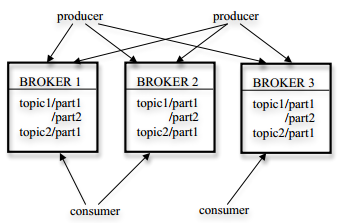
\includegraphics{figures/kafka_arch}
\caption{Kafka architecture}
\label{figure:kafka_arch}
\end{figure}

For each topic, the Kafka cluster maintains a partitioned log with the structure depicted in Figure \ref{figure:kafka_topic}. A \emph{partition} is essentially a commit log to which an ordered, immutable sequence of messages that is continually appended. Every message is assigned an offset: a sequential id number that uniquely identifies the message within the partition. Kafka only provides a total order over messages within a partition, not between different partitions in a topic.

\begin{figure}[H]
\centering
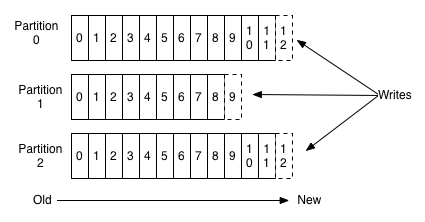
\includegraphics{figures/kafka_topic}
\caption{Kafka topic structure}
\label{figure:kafka_topic}
\end{figure}

All published messages remain stored at the brokers for a configurable period of time, whether or not they have been consumed. Kafka's performance is effectively constant with respect to data size, allowing a big volume of data to be retained. The only metadata retained for each consumer is the offset of the consumer in the log. By controlling this offset the consumer can read messages in any order. For example a consumer can advance its offset linearly as it reads messages or even reset to an older offset to reprocess them.

The partitions in the log serve several purposes. Firstly, they allow the log to scale in size, by being distributed over the brokers of the cluster. Moreover, the partitions are replicated across a configurable number of brokers to provide fault tolerance. For each partition one broker acts as the leader,  handling all the requests for the partition, and zero or more brokers act as followers, replicating the leader. Finally, partitions act as the unit of parallelism and provide load balancing over the write and read requests of the producers and the consumers respectively.


\section{Storm}

\subsection{Introduction}

Storm is a real-time fault-tolerant and distributed stream data processing system. It was originally created by BackType and was subsequently open sourced after being acquired by Twitter in 2011. Storm is an Apache Top-Level Project since 2014. The basic Storm data processing architecture consists of streams of tuples flowing through topologies. A topology is a directed graph where the vertices represent computation and the edges represent the data flow between the computation components. Vertices are divided into spouts and bolts, that define information sources and manipulations respectively.

Storm demonstrates the following key properties:
\begin{itemize}
\item \textbf{Scalable:} Storm topologies are inherently parallel and run across a cluster of machines. Different parts of a topology can be scaled individually by tweaking their parallelism. Moreover, nodes can be added or removed from the Storm cluster without disrupting the existing topologies.
\item \textbf{Resilient:} Storm is designed to be fault-tolerant. If there are faults or failures during the execution of a topology, Storm will reassign tasks as necessary.
\item \textbf{Efficient:} Storm must have good performance characteristics, since it is used in real-time applications. To achieve this Storm uses a number of techniques, including keeping all its storage and computational data structures in memory.
\item \textbf{Reliable:} Storm guarantees every tuple will be fully processed by tracking the lineage of every tuple as it advances through the topology.
\item \textbf{Easy to monitor:} Storm provides easy-to-use administration tools that help end-users immediately notice if there are failure or performance issues associated with Storm.
\end{itemize}

\subsection{Storm Architecture}

A Storm cluster consists of one master node and one or more worker nodes. The \emph{master node} runs the \emph{Nimbus} daemon that is responsible for distributing code around the cluster, assigning tasks to machines, and monitoring for failures.

Every \emph{worker node} runs a \emph{Supervisor} daemon that listens for work assigned to its machine and starts and stops \emph{worker processes} as necessary based on what Nimbus has assigned to it. Each worker process executes a subset of a topology.

\begin{figure}[H]
\centering
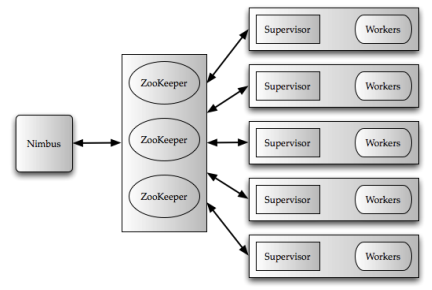
\includegraphics[width=0.8\textwidth]{figures/storm_cluster}
\caption{Storm architecture}
\label{figure:storm_cluster}
\end{figure}

All coordination between Nimbus and the Supervisors is done through a Zookeeper cluster. Additionally, the Nimbus daemon and Supervisor daemons are fail-fast and stateless, because all state is kept in Zookeeper or on local disk. This design leads to Storm clusters being incredibly stable, allowing the cluster to recover even if Nimbus or the Supervisors are killed and restarted afterwards.

\subsection{Topologies}

The core abstraction in Storm is the \emph{stream}, an unbounded sequence of tuples. A \emph{tuple} is a named list of values, and a field in a tuple can be an object of any type. The basic primitives Storm provides for doing stream transformations are spouts and bolts.

A \emph{spout} is a source of streams in a computation. Usually a spout reads from a queueing broker such as Kafka, but a spout can also generate its own stream or read from a streaming API.

A \emph{bolt} consumes any number of input streams, does some processing, and possibly emits new streams.  Most of the logic of a computation goes into bolts, such as functions, filters, streaming joins, streaming aggregations, databases queries, etc.

Networks of spouts and bolts are packaged into a topology which is the top-level abstraction is submitted to Storm clusters for execution. A \emph{topology} is a graph of stream transformations where each vertex is a spout or bolt. Edges in the graph indicate which bolts are subscribing to which streams. Topologies run indefinitely when deployed.

\begin{figure}[H]
\centering
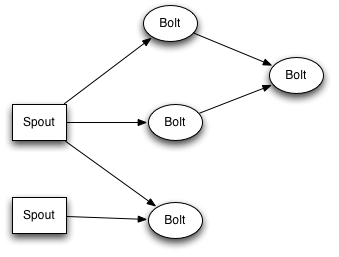
\includegraphics{figures/storm_topology}
\caption{Example storm topology}
\label{figure:storm_topology}
\end{figure}

Each component (spout or bolt) in a Storm topology executes in parallel. The degree of parallelism for each component can be configured and Storm will spawn that number of threads across the cluster to do the execution.

\subsection{Parallelism in Storm}

There are three main entities that are used to actually run a topology in a Storm cluster: worker processes, executors and tasks. The relationships between them are illustrated in Figure \ref{figure:storm_parallelism}.

\begin{figure}[H]
\centering
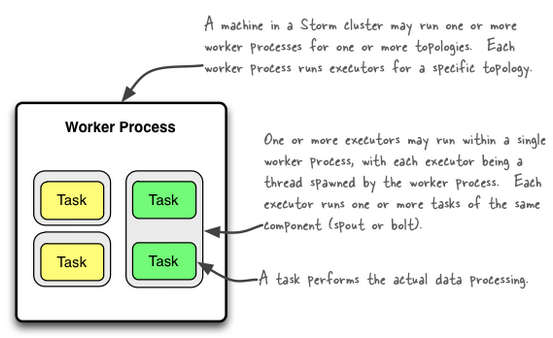
\includegraphics[width=0.8\textwidth]{figures/storm_parallelism}
\caption{The relationships between worker processes, executors and tasks}
\label{figure:storm_parallelism}
\end{figure}

A \emph{worker process} runs a JVM and executes a subset of a topology. Each worker process belongs to a specific topology and may run one or more executors.

An \emph{executor} is a thread spawned by a worker and may run one or more tasks for the same topology component. All of the tasks belonging to the same executor are run serially, since every executor always corresponds to one thread.

A \emph{task} performs the actual data processing for a topology component. Each spout or bolt is executed as many tasks across the cluster. The number of tasks for a component is static, in contrast to the number of executors for a component that can be changed after the topology has been started. By default, Storm will run one task per executor.

\subsection{Stream Groupings}

A \emph{stream grouping} defines how a stream between two components (spout to bolt or bolt to bolt) is partitioned among the tasks of each component. For example, the way tuples are emitted between the sets of tasks corresponding to Bolt A and Bolt B in Figure \ref{figure:storm_groupings} is defined by a stream grouping.

\begin{figure}[H]
\centering
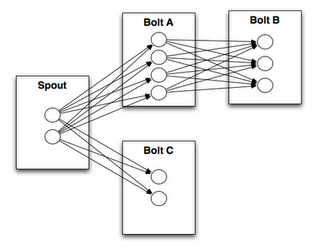
\includegraphics{figures/storm_groupings}
\caption{Task-level execution of a topology}
\label{figure:storm_groupings}
\end{figure}

Storm supports the following stream groupings:
\begin{itemize}
\item \textbf{Shuffle grouping:} Tuples are randomly and evenly distributed across the bolt's tasks.
\item \textbf{Fields grouping:} The stream is partitioned by the fields specified in the grouping. This guarantees that tuples with the same values on the specified fields are emitted to the same task.
\item \textbf{All grouping:} The stream is replicated across all the bolt's tasks.
\item \textbf{Global grouping:} The entire stream goes to a single one of the bolt's tasks.
\item \textbf{Local grouping:} If there are one or more of the bolt's tasks in the same worker process, tuples will be shuffled to just those in-process tasks.
\end{itemize}

\section{Hadoop Distibuted File System}

The Hadoop Distributed File System (HDFS) is a distributed file system designed to run on commodity hardware, inspired by the Google File System. It can reliably store very large files across machines in a large cluster and provides high throughput access to large data sets. HDFS is the storage part of the Hadoop framework, an Apache Top-Level Project since 2006.

Each file on HDFS is stored as a sequence of blocks of the same size, except the last block. Blocks belonging to a file are replicated for fault tolerance. The block size and replication factor are configurable per file.

HDFS has a master/slave architecture. An HDFS cluster consists of a single NameNode and one DataNode per node in the cluster. \emph{NameNode} is a master server that manages the file system namespace and regulates access to files by clients. Each \emph{DataNode} manages storage attached to the node that it run on. HDFS exposes a file system namespace and allows user data to be stored in files. Every file is split into blocks that are stored in a set of DataNodes. The NameNode determines the mapping of blocks to DataNodes and executes file system namespace operations like opening, closing, and renaming files and directories. The DataNodes are responsible for serving read and write requests from the file system’s clients and also perform block creation, deletion, and replication upon instruction from the NameNode.

\begin{figure}[H]
\centering
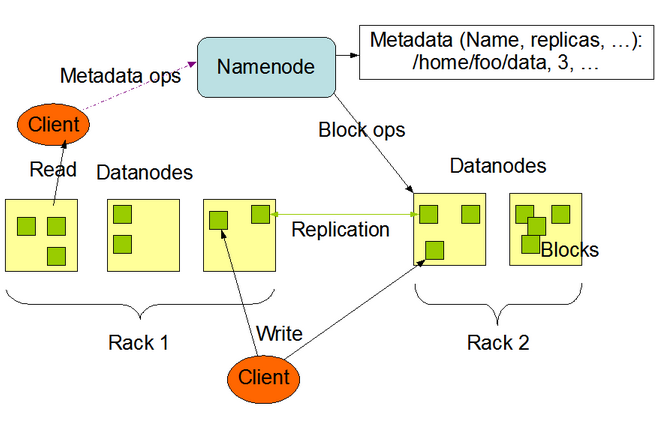
\includegraphics[width=0.8\textwidth]{figures/hdfs_architecture}
\caption{HDFS architecture}
\label{figure:hdfs_architecture}
\end{figure}


\section{HBase}

\subsection{Introduction}

HBase is a distributed non-relational database modeled after Google's BigTable, that runs on top of the HDFS. It provides a fault-tolerant way of storing large quantities of sparse data, while allowing random, real-time access to them. HBase is an Apache Top-Level Project since 2010.

HBase offers the following key features:
\begin{itemize}
\item \textbf{Linear and modular scalability:} HBase clusters expand by adding RegionServers that are hosted on commodity class servers, increasing storage and as well as processing capacity.
\item \textbf{Strictly consistent reads and writes:} HBase guarantees that all writes happen in an order, and all reads are seeing the most recent committed data.
\item \textbf{Automatic sharding of tables:} HBase tables are distributed on the cluster via regions, and regions are automatically split and re-distributed as data grows.
\item \textbf{Automatic failover support between RegionServers:} If a RegionServers fails, the regions it was hosting are reassigned between the available RegionServers.
\item \textbf{Integration with Hadoop MapReduce:} HBase supports massively parallelized processing via MapReduce for using HBase as both source and sink.
\item \textbf{Block Cache and Bloom Filters:} HBase supports a Block Cache and Bloom Filters for real-time queries.
\end{itemize}

\subsection{HBase Data Model}

The data model of HBase is very different from that of relational databases. As described in the  Bigtable paper, it is a sparse, distributed, persistent multidimensional sorted map. The map is indexed by a row key, column key, and a timestamp.

\begin{gather*}
(rowkey, column, timestamp) \rightarrow value
\end{gather*}

The basic elements of the HBase data model and the relations between them are presented below:
\begin{itemize}
\item \textbf{Table:} HBase organizes data into tables.
\item \textbf{Row:} Within a table, data is stored according to its row. A row consists of a row key and one or more columns with values associated with them. Rows are identified uniquely and sorted alphabetically by their row key.
\item \textbf{Column:} A column consists of a column family and a column qualifier, which are delimited by a : (colon) character.
\item \textbf{Column Family:} Data within a row is grouped by column family. Column families physically colocate a set of columns and their values. Each column family has a set of storage properties. For these reasons, column families must be declared up front at schema definition. Every row in a table has the same column families, though a given row might not store data in all of its families.
\item \textbf{Column Qualifier:} Data within a column family is addressed via its column
qualifier. Though column families are fixed at table creation, column qualifiers are mutable and may differ greatly between rows.
\item \textbf{Cell:} A combination of row, column family, and column qualifier uniquely identifies a cell. The data stored in a cell is that cell's value.
\item \textbf{Timestamp:} Values within a cell are versioned. A timestamp is written alongside each value, and is the identifier for a given version of a value.
\end{itemize}

\begin{figure}[H]
\centering
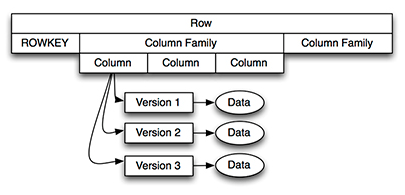
\includegraphics{figures/hbase_data_model}
\caption{HBase data model}
\label{figure:hbase_data_model}
\end{figure}

There are four primary data model operations in HBase:
\begin{itemize}
\item \textbf{Get:} Returns the values for a specified row.
\item \textbf{Put:} Adds a row to a table, if the key is new. If the key already exists, the row is updated.
\item \textbf{Scan:} Returns the values for a range of rows. Filters can also be used to narrow down the results.
\item \textbf{Delete:} Marks a row for deletion by adding a Tombstone marker. These rows are cleaned up during the next major compactions of the table.
\end{itemize}

\subsection{HBase Architecture}

In HBase, tables are are divided horizontally by row key range into \emph{regions}. Regions are vertically divided by column families into \emph{stores}, which are saved as files in HDFS (\emph{HFiles}). Figure \ref{figure:hbase_architecture} illustrates the architecture of HBase.

\begin{figure}[H]
\centering
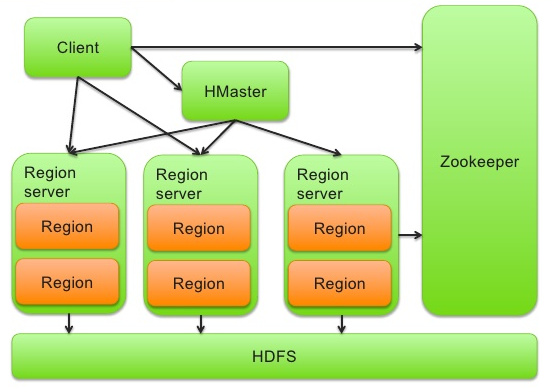
\includegraphics[width=0.8\textwidth]{figures/hbase_architecture}
\caption{HBase architecture}
\label{figure:hbase_architecture}
\end{figure}

An HBase cluster is composed of two types of servers in a master/slave type architecture. The \emph{HMaster} is responsible for monitoring all RegionServer instances in the cluster, and is the interface for all metadata changes. \emph{RegionServers} are responsible for serving and managing regions. They are collocated with the HDFS DataNodes, which enables data locality for the data served by the RegionServers. HBase uses ZooKeeper as a distributed coordination service to maintain server state in the cluster. Zookeeper maintains which servers are alive and available, and provides server failure notification.

Every RegionServer has the following components:
\begin{itemize}
\item \textbf{WAL:} Write Ahead Log is used to store new data that hasn't yet been persisted to permanent storage. The WAL is used for recovery in the case of failure.
\item \textbf{BlockCache:} Keeps data blocks resident in memory after they are read. Least Recently Used data is evicted when full.
\item \textbf{MemStore:} Stores in-memory new data which has not yet been written to disk. There is one MemStore per column family per region. Once the MemStore fills, its contents are written to disk as additional HFiles.
\item \textbf{Hfile:} Stores the rows as sorted key-values on disk.
\end{itemize}

\begin{figure}[H]
\centering
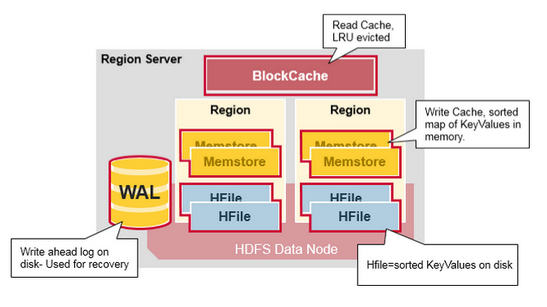
\includegraphics[width=0.8\textwidth]{figures/hbase_regionserver_components}
\caption{RegionServer components}
\label{figure:hbase_regionserver_components}
\end{figure}


\section{Phoenix}

\subsection{Introduction}

Apache Phoenix is relational database layer for HBase, targeting low latency queries over HBase data. Phoenix provides a JDBC driver that hides the intricacies of Hbase enabling users to create, delete, and alter SQL tables, views, indexes, and sequences, upsert and delete rows singly and in bulk and query data through SQL. Phoenix began as an internal project by the company Salesforce and was subsequently open-sourced and became a top-level Apache project on 2014.

\subsection{Phoenix Data Model}

The relational elements of the Phoenix data model are mapped to their respective counterparts in the HBase data model:

\begin{itemize}
\item A Phoenix table is mapped to an HBase table.
\item The Phoenix table's columns that are included in the primary key constraint are mapped together to the HBase row key.
\item The rest of the columns are mapped to HBase columns, consisting of a column family and a column qualifier.
\end{itemize}

Columns in a Phoenix table are assigned an SQL datatype. Phoenix serializes data from their datatype to byte arrays when upserting, because HBase stores everything as a byte array. In this way Phoenix allows typed access to HBase data.

\subsection{Phoenix Architecture}

On the client-side Phoenix is a JDBC driver that hides an HBase client from the user. The Phoenix driver compiles queries and other statements into native HBase client calls, enabling the building of low latency applications.

On the server-size a Phoenix jar is installed in every RegionServer, allowing Phoenix to take advantage of coprocessors and custom filters that HBase provides in order to increase performance. Coprocessors perform operations on the server-side thus minimizing client/server data transfer and custom filters prune data as close to the source as possible.

\begin{figure}[H]
\centering
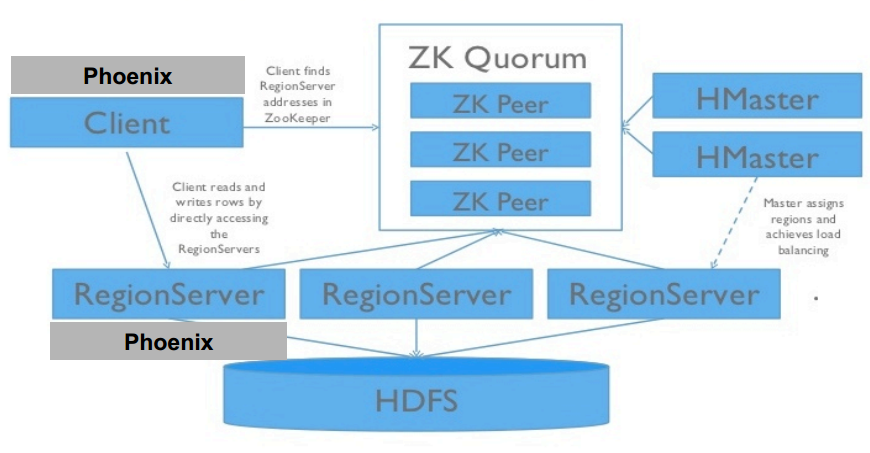
\includegraphics[width=0.8\textwidth]{figures/phoenix_architecture}
\caption{Phoenix and HBase architecture}
\label{figure:phoenix_architecture}
\end{figure}

\subsection{TopN Queries}

TopN queries return the top N rows, where top is determined by the \texttt{ORDER BY} clause and N is defined by the \texttt{LIMIT} clause of the SQL query. An example topN query for a pair of columns is presented below.

\begin{lstlisting}[language=PhoenixSQL]
SELECT column1, column2, COUNT(*) AS pairCount
FROM table
WHERE column3 > 0
GROUP BY column1, column2
ORDER BY pairCount DESC
LIMIT 10;
\end{lstlisting}

The execution of this query needs to make a pass through all the rows restricted by the \texttt{WHERE} clause and sort the results of the \texttt{GROUP BY}, which is very computationally expensive  for large tables. In order to decrease execution time, Phoenix handles these queries in a different way, using an approximate algorithm described below.

Firstly, the Phoenix client issues parallel scans restricted by the \texttt{WHERE} clause of the query. The parallel scans are \emph{chunked} by region boundaries and guideposts. \emph{Guideposts} are a set of keys per region per column family collected by Phoenix at an equal byte distance from each other, that act as hints to improve the parallelization of queries on their region. The rows that satisfy the \texttt{WHERE} clause are grouped for each chunk in parallel on the server-side by the topN coprocessor, according to the \texttt{GROUP BY} clause. The topN coprocessor of each RegionServer keeps only the top N rows for each chunk. Afterwards, the Phoenix client receives the top N rows for each chunk, does a final merge sort and returns the top N rows.


\cleardoublepage

\chapter{System Description}\label{chapter:system}

\section{System Overview}

As mentioned before, the objective of this thesis is the design and implementation of a distributed system that allows the execution of SQL queries that join a real-time data stream and an external dataset. The prerequisites for the system are scalability, fault tolerance, extensibility, but most importantly enabling the execution of low latency SQL queries. This means that the latency between the issue of the query and the moment we receive the query response must be minimized. The delay between the data generation and the moment they are available for querying must also be as small as possible, since we are dealing with a real-time data stream.

Performing an SQL join combines records from two tables. The join effectively creates a third table which combines the information from both of them. Performing a join can be expensive in terms of the time it takes to compute it, especially if one or both of the tables are large in size. Since minimizing the join query latency is our priority, we can store the stream of data combined with the external data information in a single denormalized table. \emph{Denormalization} is the process of attempting to optimize the read performance of a database by adding redundant data, an example of which can be seen in Table \ref{table:denormalization_example}. A Storm topology can compute the join of the data stream and the external dataset in real time and store the denormalized data stream at a Phoenix table in HBase.

\begin{table}[h!]
\centering
\subfloat[Employee table]{\begin{tabular}{ |c|c| }
\hline
LastName & DepartmentID \\ \hline \hline
Jones & 2 \\ \hline
Wagner & 1 \\ \hline
Gray & 1 \\ \hline
Draper & 3 \\ \hline
Nolan & 2 \\ \hline
\end{tabular}}
\quad
\subfloat[Department table]{\begin{tabular}{ |c|c| }
\hline
DepartmentID & DepartmentName \\ \hline \hline
1 & Sales \\ \hline
2 & Engineering \\ \hline
3 & Marketing \\ \hline
\end{tabular}}
\\
\subfloat[Denormalized table]{\begin{tabular}{ |c|c|c| }
\hline
LastName & DepartmentID & DepartmentName \\ \hline \hline
Jones & 2 & Engineering\\ \hline
Wagner & 1 & Sales\\ \hline
Gray & 1 & Sales\\ \hline
Draper & 3 & Marketing\\ \hline
Nolan & 2 & Engineering\\ \hline
\end{tabular}}
\caption{Denormalization example}
\label{table:denormalization_example}
\end{table}

This design decision allows all subsequent queries that combine the data stream and the external dataset to be performed directly on the denormalized Phoenix table, without the need to perform the computationally expensive join on query time. Denormalization introduces a trade-off, speeding up reads from queries while slowing down writes to the table, since the join is performed by the Storm topology. However, if the system processing rate can handle the real-time data generation rate, slower writes are not a problem.

From a high level, the system implemented for our IXP network data use case consists of 4 major parts that can be seen in Figure \ref{figure:system_overview}. In the first part, the network data is generated by the switches of an IXP and collected by a host running a Kafka producer. There, the useful fields are extracted from the headers of the captured packets and published to the Kafka topic. The second component of the system is the Kafka topic that temporarily stores the data stream at the Kafka cluster. In the next part, the data stream is processed by a Storm topology. The topology contains the IP to AS Bolt, that performs the join of the data stream and the AS dataset in-memory, since the size of the dataset is small enough. It also contains the IP to DNS Bolt, that performs the join of the data stream and the Reverse DNS dataset using \texttt{Get} operations on the HBase table where the dataset is stored, since it does not fit in the bolt's memory. Finally, in the last part the denormalized network data is stored at a Phoenix table in HBase, allowing Phoenix clients to perform low latency SQL queries to it.

\begin{figure}[h!]
\centering
\includegraphics[width=\textwidth]{figures/system_overview}
\caption{Storm architecture overview}
\label{figure:system_overview}
\end{figure}

The system's \textbf{scalability} is achieved by using distributed frameworks and technologies for its implementation. Kafka topics consist of partitions that are distributed over a cluster of Kafka brokers. Storm topologies run over a cluster of Supervisors and multiple instances of any component of the topology (spout or bolt) can run at the same time. The output Phoenix table is stored in HBase, and subsequently in the HDFS, which are both distributed technologies that run on clusters of DataNodes and RegionServers respectively. Moreover, Phoenix can parallelize queries to take full advantage of the HBase cluster.

\textbf{Fault tolerance} is very important for our system since it will be constantly running for extended periods of time, processing real-time data. First of all, Kafka topic partitions can be replicated across multiple Kafka brokers, allowing data input by the Kafka producer and consumption by the Storm topology even in the case of a broker failure. Storm topologies are also fault-tolerant and in case of a Supervisor failure Nimbus reassigns the tasks as necessary. Storm also keeps track of failed tuples and is able to replay them, since Kafka retains a topic's data for a configurable period of time. This allows us to restart Storm topologies without skipping any data. Finally, the output Phoenix table that is stored in HBase is replicated by the underlying HDFS, allowing its data to be available in the case of a DataNode or RegionServer failure.

Using the Storm framework provides \textbf{extensibility} to our system. Extending the functionality of the Storm topology for a new dataset is as simple as adding an extra bolt to the topology. For example, the processing for the join of the data stream with a new external dataset can be added by implementing the new bolt and placing it before the output Phoenix Bolt. We discern two cases with respect to the size of the external dataset. If the dataset's size is small enough, we can load it in the bolt's memory and perform the join in-memory. Otherwise, when the dataset does not fit in memory, we store it in an HBase table and perform the join using \texttt{Get} operations.

In the following Sections of this Chapter we offer a detailed description for all of the system's components.


\section{Data Generation and Input}

\subsection{IXP Switch}

The data stream that is processed by our system is generated by an \emph{sFlow agent} running on a switch that processes traffic in an IXP. sFlow \cite{sflow} is an industry standard technology for monitoring high speed switched networks and is supported by multiple network device manufacturers. The sFlow agent performs random sampling to the packets processed by the switch. By default, the agent samples the first 128 bytes of 1 in every 2048 packets.

The flow samples are sent as \emph{sFlow datagrams} (UDP packets) to the \emph{sFlow collector}, described in Subsection \ref{subsection:system_kafka_producer}. The sFlow collector can accept sFlow datagrams from multiple sFlow agents, allowing us to process a data stream that combines flow samples generated by multiple switches that are used in the same IXP.

\subsection{Kafka Producer}\label{subsection:system_kafka_producer}

The sFlow datagrams are sent by the sFlow agents of the IXP switches to an sFlow collector running at a specified host. This sFlow collector collects the flow samples from all of the switches and makes them available for further processing. In our implementation we use \texttt{sflowtool} \cite{sflowtool}, a tool functions as an sFlow collector and translates the flow samples to a simple-to-parse ASCII format.

The same host runs a Kafka producer script that preprocesses the flow samples and publishes the useful fields to a Kafka topic. This script reads the output of our sFlow collector \texttt{sflowtool} and extracts the following useful fields for each sampled packet:
\begin{itemize}
\item \texttt{sourceIP}: source IP address in dot-decimal notation
\item \texttt{destinationIP}: destination IP address in dot-decimal notation
\item \texttt{protocol}: IP protocol number (6 for TCP, 17 for UDP)
\item \texttt{sourcePort}: source port number
\item \texttt{destinationPort}: destination port number
\item \texttt{ipSize}: total length of the IP packet
\item \texttt{dateTime}: Unix timestamp of the packet's capture time in microseconds. This field is generated by the script while preprocessing each packet. 
\end{itemize}

After the extraction, we compose a message containing the fields in CSV format. The script is running a Kafka producer that publishes these messages to the Kafka topic \texttt{netdata} that is stored at the Kafka cluster. 

Algorithm \ref{algorithm:kafka_producer} outlines the script implementation.

\begin{algorithm}[H]
\begin{algorithmic}[1]
\For {line in sFlowToolOutput}
\State fields = line.split(",")
\State sourceIP = fields[9]
\State destinationIP = fields[10]
\State protocol = fields[11]
\State sourcePort = fields[14]
\State destinationPort = fields[15]
\State ipSize = fields[17]
\State dateTime = int(time.time()*1000000)
\State message = "\{\},\{\},\{\},\{\},\{\},\{\},\{\}".format(sourceIP, destinationIP, protocol, sourcePort, destinationPort, ipSize, dateTime)
\State kafkaProducer.send\_messages("netdata", message)
\EndFor
\end{algorithmic}
\caption{Kafka Producer}
\label{algorithm:kafka_producer}
\end{algorithm}

Messages can be sent to a Kafka topic either synchronously or asynchronously \cite{kafka_documentation}. Synchronous send publishes the messages immediately, whereas asynchronous send accumulates them in memory batches multiple messages in a single request. As we will see in Subsection \ref{subsection:benchmarks_kafka_batch} batching can greatly increase the performance of the producer, therefore we choose to use asynchronous send.


\section{Kafka Topic}

The preprocessed messages containing the useful fields in CSV format are stored at the \texttt{netdata} Kafka topic in the Kafka cluster. To ensure scalability and load balancing, we set the number of the topic's partitions equal to the number of the brokers of the Kafka cluster. In this way, the write and read requests of the producer and the consumers respectively are distributed over the cluster.

To provide fault tolerance, we also set a replication factor of 2 for the topic. This means that every partition is replicated and stored in 2 brokers, the leader that handles all the requests for the partition, and the follower that is replicating the leader. In case of failure of the topic leader, the follower can take over and handle the requests for the partition.

As we mentioned in Section \ref{section:theory_kafka}, all published messages remain stored at the brokers for a configurable period of time, whether or not they have been consumed. This allows the Storm topology to replay previously read messages in case of failure. The default data retention window for the topic is 7 days.


\section{Storm Topology}

The Storm topology is the heart of our system. This is where the processing of the data stream is performed. The topology consists of one spout and four bolts in a pipeline setup: Kafka Spout, Split Fields Bolt, IP to AS Bolt, IP to DNS Bolt and Phoenix Bolt. In short, the topology reads messages from a Kafka topic, extracts the useful fields from the messages, performs the join of the data stream and the external datasets and finally stores the denormalized data stream in a Phoenix table. The topology has acking enabled, which guarantees that every message from the topic will be processed and will be replayed in case of failure.

The overview of the Storm topology for our network data use case can be seen in Figure \ref{figure:system_storm_topology}. The functionality of the topology can be extended by adding more bolts that perform the join of the data stream and another external dataset right before the Phoenix Bolt.

\begin{figure}[h!]
\centering
\includegraphics[width=\textwidth]{figures/system_storm_topology}
\caption{Storm topology overview}
\label{figure:system_storm_topology}
\end{figure}

\subsection{Kafka Spout}

The source of data stream in our topology is the Kafka Spout. The spout is a Kafka consumer that reads messages from the \texttt{netdata} Kafka topic and emits them to the Split Fields Bolt. The maximum parallelism of the Kafka spout is the number of the topic's partitions, because any instances of the spout further than that would not read any data.

The Kafka Spout stores the offset of the consumer for each partition of the topic in Zookeeper. In this way, if a failure happens the topology can be restarted and resume reading messages from the last one that was executed successfully by the topology.

\subsection{Split Fields Bolt}

The tuple emitted by the Kafka Spout has a single field: a message from the topic containing the useful fields of the packet in CSV format. The Split Fields Bolt extracts these fields from the message. In addition to that the bolt computes the integer representations of the source and destination IP addresses, which are usually more useful than the IP addresses in dot-decimal notation.

After processing the Kafka message, the Split Fields Bolt emits a tuple containing the following fields: sourceIP, sourceIPInt, destinationIP, destinationIPInt, protocol, sourcePort, destinationPort, ipSize, dateTime.

\subsection{IP to AS Bolt}

The join of the data stream and the Autonomous System dataset is performed by the IP to AS Bolt. The Autonomous System dataset maps IP address ranges to AS number and name. The data contained in the dataset are stored in CSV format and have 3 fields: the first IP address contained in the AS, the last IP address contained in the AS and the AS number and name. The IP addresses are stored in their integer representation format. The dataset file must be stored in a location accessible by all of the Supervisors, such as the HDFS. Further information on the dataset is available in Subsection \ref{subsection:benchmarks_as_dataset}.

The defining characteristic of the Autonomous System dataset is that its size (13 MB) is small enough to fit in the memory, which is the optimal way to perform the join of the stream and the dataset. During the initialization of the topology the \texttt{prepare} method of the IP to AS Bolt is called and loads the dataset in a TreeMap structure. A TreeMap is a map implementation based on red-black trees, a variation of binary search trees, that allow searching in $O(\log{n})$ time \cite{treemap}. For each record of the dataset we insert two records in the TreeMap, containing the start and the stop IP address for each AS along with the AS number and name, as seen in Algorithm \ref{algorithm:ip_to_as_bolt}.

\begin{algorithm}[H]
\begin{algorithmic}[1]
\Function{prepare}{}
\State asMap = new TreeMap<Long, String[]>()
\For {line in ipToASFile}
\State fields = line.split(",")
\State asMap.put(fields[0], [fields[2], "start"])
\State asMap.put(fields[1], [fields[2], "stop"])
\EndFor
\EndFunction

\Function{ipToAS}{ipInt}
\State as = "null"
\State key = asMap.ceilingKey(ipInt)
\If {key != null}
\State value = asMap.get(key)
\If {(key == ipInt) || (value[1].equals("stop"))}
\State as = value[0]
\EndIf
\EndIf
\Return as
\EndFunction

\Function{execute}{tuple}
\State sourceIPInt = tuple.getField("sourceIPInt")
\State destinationIPInt = tuple.getField("destinationIPInt")
\State outputValues = tuple.getValues()
\State outputValues.add(ipToAS(sourceIPInt))
\State outputValues.add(ipToAS(destinationIPInt))
\State collector.emit(outputValues)
\EndFunction
\end{algorithmic}
\caption{IP to AS Bolt}
\label{algorithm:ip_to_as_bolt}
\end{algorithm}

The helper method \texttt{ipToAS} takes an IP address in integer representation format as input and returns the name and number of the AS it belongs. More specifically, by using the TreeMap's \texttt{ceilingKey} and \texttt{get} methods we find the first AS boundary IP address larger or equal to the input IP address. If this address is equal to the input IP address or corresponds to the last address of an AS IP address range, then the AS it belongs is the one we are looking for and its number and name is returned by the method. Otherwise the IP address provided does not belong to any AS according to the dataset and the \texttt{ipToAS} method returns the String \texttt{"null"}.

For every tuple received by the bolt, the \texttt{execute} method is called. Using the sourceIPInt and destinationIPInt fields as input to the method \texttt{ipToAS} we determine the sourceAS and destinationAS fields that denote the source and destination AS number and name respectively. The new fields are appended to the received fields and all of them are emitted to the next bolt of the topology.

\bigskip

\subsection{IP to DNS Bolt}

The join of the data stream and the Reverse DNS dataset is performed by the IP to DNS Bolt. The Reverse DNS dataset maps IP addresses to domain names. The data contained in the dataset have 2 fields: the IP address in dot-decimal notation and the corresponding domain name. Further information on the dataset is available in Subsection \ref{subsection:benchmarks_dns_dataset}.

The defining characteristic of the Reverse DNS dataset is that its size (55 GB uncompressed) is larger than the memory size, therefore loading it in every bolt's memory is not an option. To make the dataset available to the bolts, we store it in the \texttt{rdns} HBase table, where the IP addresses are used as the row key and the domain names are stored in the column \texttt{d:dns}. This allows the bolt to perform \texttt{Get} operations on the table for an IP address row key to receive the corresponding domain name.

HBase can perform low latency \texttt{Get} operations by using \emph{Bloom filters} \cite{bloom}. A Bloom filter, is a data structure which is designed to predict whether a given element is a member of a set of data. A positive result from a Bloom filter is not always accurate, but a negative result is guaranteed to be accurate. In HBase, Bloom filters a lightweight in-memory structure that reduces the number of disk reads for a given \texttt{Get} operation to only the HFiles likely to contain the desired row.

The helper method \texttt{ipToDNS} takes an IP address in dot-decimal notation as input and returns corresponding domain name. More specifically, a \texttt{Get} operation is performed on the \texttt{rdns} HBase table for the input IP address row key. If the \texttt{Get} is successful, the corresponding domain name is the value of the column \texttt{d:dns} of the returned row, and is afterwards returned by the method. Otherwise the IP address provided does not have a corresponding domain name according to the dataset and the \texttt{ipToDNS} method returns the String \texttt{"null"}.

For every tuple received by the bolt, the \texttt{execute} method is called. Using the sourceIP and destinationIP fields as input to the method \texttt{ipToDNS} we determine the sourceDNS and destinationDNS fields that denote the source and destination domain names respectively. The new fields are appended to the received fields and all of them are emitted to the next bolt of the topology.

Algorithm \ref{algorithm:ip_to_dns_bolt} outlines the IP to DNS Bolt implementation.

\begin{algorithm}[H]
\begin{algorithmic}[1]
\Function{ipToDNS}{ip}
\State table = new HTable("rdns")
\State g = new Get(ip)
\State res = table.get(g)
\State dns = res.getValue("d", "dns")
\If {dns == null}
\State dns = "null"
\EndIf
\Return dns
\EndFunction

\Function{execute}{tuple}
\State sourceIP = tuple.getField("sourceIP")
\State destinationIP = tuple.getField("destinationIP")
\State outputValues = tuple.getValues()
\State outputValues.add(ipToDNS(sourceIP))
\State outputValues.add(ipToDNS(destinationIP))
\State collector.emit(outputValues)
\EndFunction
\end{algorithmic}
\caption{IP to DNS Bolt}
\label{algorithm:ip_to_dns_bolt}
\end{algorithm}

\subsection{Phoenix Bolt}

The last component of the topology is the Phoenix Bolt, which inserts the denormalized data stream into the \texttt{netdata} Phoenix table. The table is described in detail in Section \ref{section:system_phoenix_table}. This bolt uses the Phoenix JDBC driver and performs an \texttt{UPSERT VALUES} query that includes all the fields received by the bolt. \texttt{UPSERT} queries are the only way to insert data in a table in Phoenix. This query inserts the row if not present, otherwise it updates the row's values in the table. In our case where the primary key of the table is the packet timestamp which is monotonically increasing this query behaves like \texttt{INSERT VALUES}.

\begin{lstlisting}[language=PhoenixSQL]
UPSERT INTO netdata VALUES (dateTime, sourceIP, sourceIPInt, destinationIP, destinationIPInt, protocol, sourcePort, destinationPort, ipSize, sourceAS, destinationAS, sourceDNS, destinationDNS);
\end{lstlisting}


\section{Phoenix Table}\label{section:system_phoenix_table}

After being computed by the Storm topology, the denormalized data stream is stored at the \texttt{netdata} Phoenix table in HBase. The design of this table is important because it affects the way queries are executed. In our use case, the queries performed will be topN AS or topN DNS queries over a time window for the data. 

The queries performed on the table have a time window constraint. To benefit from HBase \texttt{Scan} operations that perform sequential reads, we want to use the packet's capture timestamp as the row key in the underlying HBase table. In this way, the HBase table is sorted by capture timestamp and the data for any time window are stored sequentially. To achieve this in Phoenix, we use the packet's capture timestamp as the primary key of the Phoenix table. The capture timestamp in microseconds can be used as the primary key since it is unique for each packet.

The use case queries concern either AS or DNS information. In HBase only the column families needed for the query are cached. Having separate column families containing AS, DNS and other information reduces query latency by reducing the data that have to be cached during each query \cite{hbase_reference}. Therefore we separate the table's columns in 3 column families: one for the AS fields, another for DNS fields and a default column family that contains the rest of the packet's fields.

In HBase every cell value is always (when stored, transferred or cached) accompanied by its row key, column name and timestamp. Since the table will store millions of cells the column names will be repeated several millions of times in our data \cite{hbase_reference}. This means that if the column names are large then the table size will be significantly increased. This is why we try to minimize the column names by keeping the column family and column qualifier names as small as possible.

Another way to reduce the table size is by utilizing Phoenix \emph{data types}. Using the appropriate data type for each column reduces the size of each row, which improves query performance. For example, instead of storing the capture timestamp as string, we use the \texttt{BIGINT} type. The current UNIX timestamp in microseconds has 16 digits. As a string this needs 16 bytes to be stored, whereas a \texttt{BIGINT} needs only 8 bytes.

Having all the aforementioned design choices taken into consideration we create the \texttt{netdata} Phoenix table with the columns listed below. The dots in the column names separate the column families from the column qualifiers created in the underlining HBase table.
\begin{itemize}
\item \texttt{t}: Unix timestamp of the packet's capture time in microseconds, used as the primary key
\item \texttt{d.ipS}: source IP address in dot-decimal notation
\item \texttt{d.ipSI}: integer representation of the source IP address
\item \texttt{d.ipD}: destination IP address in dot-decimal notation
\item \texttt{d.ipDI}: integer representation of the destination IP address
\item \texttt{d.proto}: IP protocol number of the packet
\item \texttt{d.portS}: source port number
\item \texttt{d.portD}: destination port number
\item \texttt{d.size}: total length of the IP packet
\item \texttt{as.asS}: AS number and name of the source IP address
\item \texttt{as.asD}: AS number and name of the destination IP address
\item \texttt{dns.dnsS}: domain name of the source IP address
\item \texttt{dns.dnsD}: domain name of the destination IP address
\end{itemize}

The Phoenix SQL statement used to create the final \texttt{netdata} table, including the optimizations that will be described in Chapter \ref{chapter:optimizations}, is the following.

\begin{lstlisting}[language=PhoenixSQL]
CREATE TABLE netdata (
    t BIGINT PRIMARY KEY,
    d.ipS VARCHAR,
    d.ipSI BIGINT,
    d.ipD VARCHAR,
    d.ipDI BIGINT,
    d.proto SMALLINT,
    d.portS INTEGER,
    d.portD INTEGER,
    d.size INTEGER,
    as.asS VARCHAR,
    as.asD VARCHAR,
    dns.dnsS VARCHAR,
    dns.dnsD VARCHAR
) 
SALT_BUCKETS = 4,
DEFAULT_COLUMN_FAMILY = 'd',
DATA_BLOCK_ENCODING = 'NONE',
COMPRESSION = 'SNAPPY';
\end{lstlisting}


\cleardoublepage

\chapter{HBase and Phoenix Optimizations}\label{chapter:optimizations}

\section{HDFS Short-Circuit Local Reads}\label{section:optimizations_short_circuit}

In the HDFS, all reads normally go through the DataNode. When a RegionServer asks the DataNode to read a file, the DataNode reads that file from the disk and sends the data to the RegionServer over a TCP socket. The downside of this approach for local reads is the overhead of the TCP protocol in the kernel, as well as the overhead of DataTransferProtocol used for the communication with the DataNode.

When the RegionServer is co-located with the data and \emph{short-circuit local reads} are enabled, local reads bypass the DataNode \cite{hadoop_short-circuit,cloudera_short-circuit}. This allows the RegionServer to read the data directly from the local disk. Short-circuit local reads provide a substantial performance boost in data transfer from the disk to the BlockCache when the data is local.

We evaluate the effect of enabling HDFS short-circuit local reads in Subsection \ref{subsection:benchmarks_hbase_short_circuit}.


\section{Compression and Data Block Encoding}\label{section:compression_encoding}

Physical data size on disk can be decreased by using compression and data block encoding \cite{hbase_reference}. \emph{Compression} reduces the size of large opaque byte arrays in cells and can significantly reduce the storage space needed to store uncompressed data. \emph{Data block encoding} attempts to limit duplication of information in keys, taking advantage of some of the fundamental designs and patterns of HBase, such as sorted row keys and the schema of a given table. Compression and data block encoding can be used together on the same column family.

Aside from on-disk data size, compression and data block encoding can reduce the data size in the BlockCache. Data is cached by default on their encoded format. In addition to that, compressed BlockCache can be enabled, allowing compressed data to be cached in their compressed and encoded on-disk format.

Between all of our compression options, Snappy \cite{snappy} is the most fitting to our use case, since minimizing query latency is our priority. It does not aim for maximum compression, but instead aims for very high speeds and reasonable compression. Compared to gzip, Snappy is an order of magnitude faster for most inputs, but the compression ratio is 20\% to 100\% lower. 

Regarding data block encoding, Fast Diff \cite{hbase_reference} is enabled by default in HBase. The format in which non-encoded data are stored in the HFile often results in multiple similar keys for each row, as seen in Figure \ref{figure:optimizations_no_encoding}.

\begin{figure}[H]
\centering
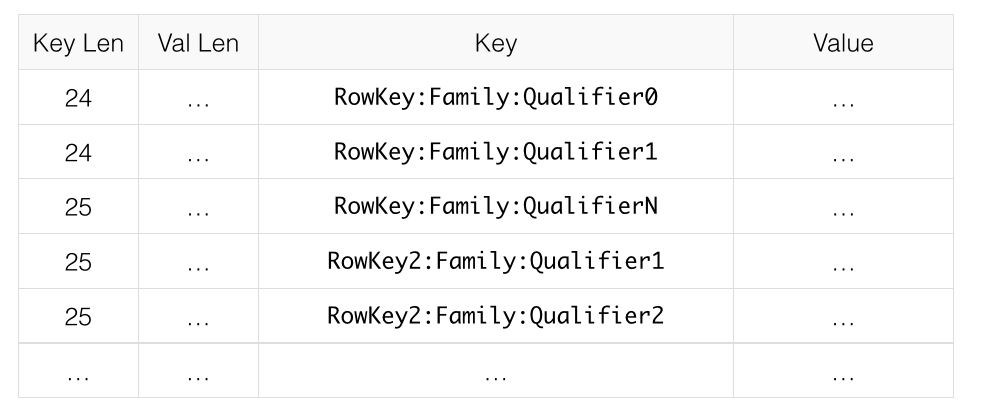
\includegraphics[width=0.7\textwidth]{figures/optimizations_no_encoding}
\caption{Column family stored with no encoding}
\label{figure:optimizations_no_encoding}
\end{figure}

Fast Diff works similar to Diff encoding, but uses a faster implementation. The most important feature of Diff encoding is an extra column which holds the length of the prefix shared between the current key and the previous key. In addition, the timestamp is stored as the difference from the previous row's timestamp, rather than being stored in full. Figure \ref{figure:optimizations_diff_encoding} shows the same data with Figure \ref{figure:optimizations_no_encoding} stored with Diff encoding.

\begin{figure}[H]
\centering
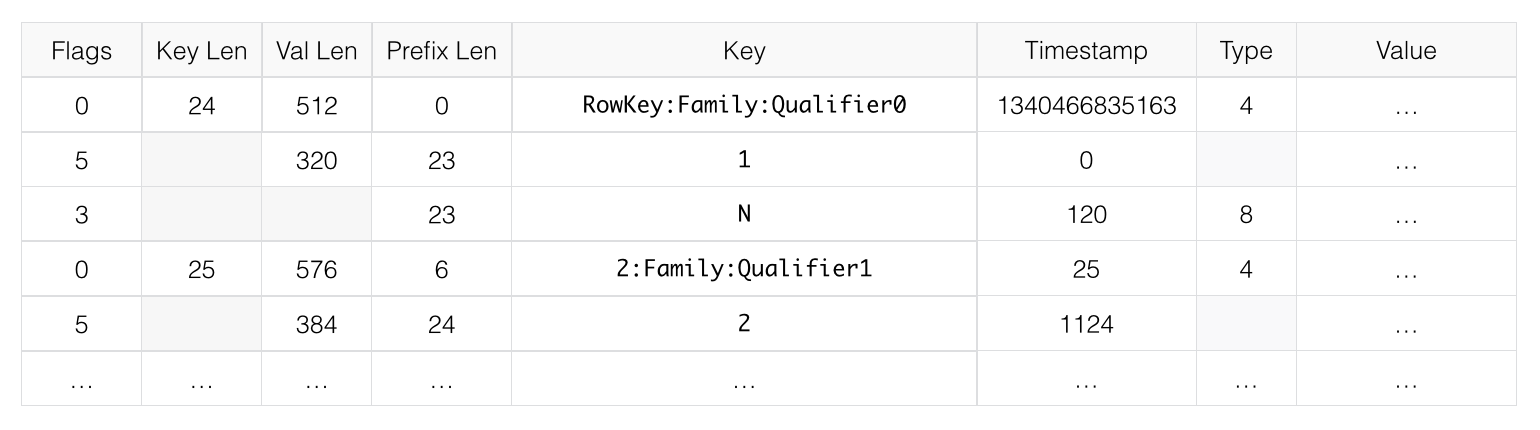
\includegraphics[width=\textwidth]{figures/optimizations_diff_encoding}
\caption{Column family stored with Diff encoding}
\label{figure:optimizations_diff_encoding}
\end{figure}

Both compression (with compressed BlockCache enabled) and data block encoding reduce the in-cache data size. This means that more rows can be cached at the same time, while data transfer time from the disk to the BlockCache for the same data is reduced. However, every time the cached data is used in a query they must be decompressed or decoded or both. These performance hits increase query latency, while is our priority is to minimize it.

To achieve the best in-cache query latency we decide to use Snappy compression for our final Phoenix table, in conjunction with enabled compressed BlockCache and no data block encoding. The experiment on which we base this decision is presented in Subsection \ref{subsection:benchmarks_compression_encoding}.


\section{Disable BlockCache on the Reverse DNS Table}

The Reverse DNS dataset is stored in the \texttt{rdns} HBase table. This table is stored with Snappy compression and no data block encoding to reduce on-disk size and avoid the decoding performance hit on read. The on-disk size of the compressed table is 12GB.

We inspect the read access pattern on the table by the IP to DNS Bolt. Since the IP addresses on the packets are random, the reads are performed on the table \texttt{rdns} are random too. Every read caches the HFile it hits, which does not provide any benefit since \texttt{rdns} does not fit into the BlockCaches of the RegionServers. Moreover, constantly caching different HFiles of \texttt{rdns} throws out of the cache HFiles of the output Phoenix table \texttt{netdata}. Subsequent queries will have to cache these HFiles again, which increases the query latency.

To alleviate this problem we disable BlockCache on \texttt{rdns}, thus allowing the \texttt{netdata} table to fully take advantage of the cache.


\section{Salting}\label{section:optimizations_salting}

Rows in HBase are sorted lexicographically by row key. The row key for the underlying HBase table where our Phoenix table is stored must be the timestamp associated with the packet, in order to optimize scans for queries over a specified time window. Since the timestamp is always increasing for live data, the row key is also monotonically increasing.

However, monotonically increasing row keys are a common source of hotspotting \cite{salting_sematext}. When records with sequential keys are being written to HBase all writes hit one Region which is served by one RegionServer. This uneven write load distribution limits the write throughput to the capacity of a single RegionServer instead of making use of multiple nodes in the HBase cluster. In addition to that, hotspotting overwhelms the RegionServer responsible for hosting that Region, causing performance degradation and potentially leading to Region unavailability.

\emph{Salting} the row key provides a way to mitigate the problem \cite{salting_phoenix,salting_sematext}. Salting refers to adding a randomly-assigned prefix to the row key, to cause it to sort differently than it otherwise would. The number of possible prefixes correspond to the number of Regions you want to spread the data across. For example we can salt the row key by using this:

\begin{lstlisting}[language=C]
newKey = (++index % BUCKETS_NUMBER) + originalKey
\end{lstlisting}

In this listing, the \texttt{newKey} is produced by prefixing the \texttt{originalKey} with a salt denoting the salt bucket. The salted records are be split into multiple buckets served by different RegionServers. The row keys of bucketed records are no longer in the original sequence, however records within in each bucket preserve their original sequence, as seen in Figure \ref{figure:optimizations_salting}.

\begin{figure}[H]
\centering
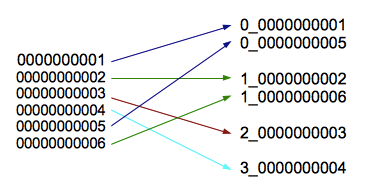
\includegraphics[width=0.6\textwidth]{figures/optimizations_salting}
\caption{HBase row key prefix salting}
\label{figure:optimizations_salting}
\end{figure}

Since data is placed in multiple buckets during writes, we have to read from all of those buckets when doing scans based on original start and stop keys and merge-sort the data. These scans can be run in parallel on the different RegionServers serving the salt buckets, which may lead to an increase in read performance.

Phoenix provides a way to transparently salt the row key with a salting byte for a particular table. To distribute the load evenly among all the nodes of the HBase cluster, we set the number of salt buckets equal to the number of the RegionServers. The effect of salting on writes and reads is evaluated in Subsections \ref{subsection:benchmarks_storm_salting} and \ref{subsection:benchmarks_hbase_salting} respectively.


\cleardoublepage

\chapter{Evaluation}\label{chapter:evaluation}

\section{Datasets}

\subsection{IXP Traffic Dataset}

The data used for the evaluation of the system is network traffic collected by GR-IX \cite{gr-ix}. GR-IX is the Greek IXP, through which ISPs exchange traffic between their networks without using their upstream transit providers. GR-IX was founded in 2009 as a successor of AIX (Athens Internet Exchange), which was in operation since 2000. The exchange is managed and operated by the Greek Research and Technology Network (GRNET).

GR-IX is handling aggregate traffic peaking at multiple Gigabytes per second. Using the packet sampling tool sFlow, IP packets were captured with a random sampling rate of 1 out of 2000 over a period of six months (July 2013 to February 2014). During this period of time 1.9 billion packets were captured, which translates to an average of 110 packets sampled per second. The captured packets were preprocessed to extract the following useful fields:
\begin{itemize}
\item \texttt{sourceIP}: source IP address in dot-decimal notation
\item \texttt{destinationIP}: destination IP address in dot-decimal notation
\item \texttt{protocol}: IP protocol number (6 for TCP, 17 for UDP)
\item \texttt{sourcePort}: source port number
\item \texttt{destinationPort}: destination port number
\item \texttt{ipSize}: total length of the IP packet
\item \texttt{dateTime}: Unix timestamp of the packet's capture time
\end{itemize}

\subsection{Autonomous System Dataset}\label{subsection:benchmarks_as_dataset}

One of the external datasets used by the topology is the GeoLite ASN IPv4 database \cite{geolite}. This dataset maps IPv4 address ranges to Autonomous System Numbers (ASN) and is updated by MaxMind every month. The dataset comes in a CSV file, having a size of 13 MB. This file is stored at HDFS in order to be available to the Storm Supervisors. The data contained in it have the following fields:
\begin{itemize}
\item \texttt{ipIntStart}: integer representation of the first IP address contained in the AS
\item \texttt{ipIntEnd}: integer representation of the last IP address contained in the AS
\item \texttt{as}: AS number and name
\end{itemize}

\subsection{DNS Dataset}\label{subsection:benchmarks_dns_dataset}

The other external dataset used by the topology is the Rapid7 Reverse DNS dataset \cite{rdns}. This dataset maps IPv4 addresses to domain names. Rapid7 Labs creates this data by performing a DNS PTR lookup for all IPv4 addresses. It is updated every 2 weeks and is made available at The Internet-Wide Scan Data Repository (scans.io). The data format is a gzip-compressed CSV file, having a size of 5.7 GB compressed and 55 GB uncompressed, while containing 1.2 billion records. The fields of the dataset are:
\begin{itemize}
\item \texttt{ip}: IP address in dot-decimal notation
\item \texttt{dns}: domain name
\end{itemize}

The Reverse DNS dataset is stored in the \texttt{rdns} HBase table. The field \texttt{ip} is used as the row key and \texttt{dns} is stored at a column.


\section{Cluster Description}

To execute the following experiments, we use virtual machines (VMs) operating on the OpenStack cluster hosted by the Computing Systems Laboratory (CSLab) of the School of Electrical and Computer Engineering, NTUA. 

For the performance tuning experiments we create 10 virtual machines:
\begin{itemize}
\item \textbf{Zookeeper:} This is a Zookeeper server in standalone mode, running the QuorumPeerMain application. Zookeeper is providing coordination between the nodes of the Kafka, Storm and HBase clusters.
\item \textbf{Master:} This node is running the master applications for all the clusters. Master runs a Nimbus daemon for Storm, a NameNode and SecondaryNameNode for HDFS and an HMaster for HBase.
\item \textbf{Storm cluster:} The Storm cluster consists of 4 virtual machines running the Supervisor daemon.
\item \textbf{Kafka and HBase cluster:} The Kafka and HBase clusters are co-hosted on 4 virtual machines. Each machine runs a Kafka server, an HDFS DataNode and HRegionServer for HBase. The RegionServer is allowed to have 5 GB of maximum heap size. Kafka CPU usage is very low during all of the benchmarks (around 3\%), therefore co-hosting it with HBase does not interfere with performance.
\end{itemize}

The deployment diagram for the clusters is presented in Figure \ref{figure:benchmarks_cluster_deployment}. Each of the virtual machines has the specifications listed in Table \ref{table:benchmarks_cluster_hw_specs}. The versions of the software used in our experiments are listed in Table \ref{table:benchmarks_cluster_sw_specs}.

To conduct the scalability experiments, we increase the number of nodes in the Storm and Kafka/ HBase clusters up to 16 for each. The rest of the deployment details remain the same.

\begin{figure}[h!]
\centering
\includegraphics[width=\textwidth]{figures/benchmarks_cluster_deployment}
\caption{Cluster deployment diagram}
\label{figure:benchmarks_cluster_deployment}
\end{figure}

\begin{table}[h!]
\centering
\begin{tabular}{ |c|c| }
\hline
Component & Description \\ \hline \hline
CPU & 4 cores @ 2.4 GHz \\ \hline
RAM & 8 GB \\ \hline
Disk & 80 GB \\ \hline
\end{tabular}
\caption{Virtual machine hardware specifications}
\label{table:benchmarks_cluster_hw_specs}
\end{table}

\begin{table}[h!]
\centering
\begin{tabular}{ |c|c| }
\hline
Software & Version \\ \hline \hline
Zookeeper & 3.4.6 \\ \hline
Kafka & 2.10-0.8.2.1 \\ \hline
Storm & 0.9.4 \\ \hline
Hadoop & 2.6.0 \\ \hline
HBase & 1.1.0.1 \\ \hline
Phoenix & 4.4.0-HBase-1.1 \\ \hline
\end{tabular}
\caption{Software versions}
\label{table:benchmarks_cluster_sw_specs}
\end{table}


\section{Kafka Performance and Scalability}

To measure Kafka performance and scalability we use the performance tools ProducerPerformance and TestEndToEndLatency shipped with the Kafka installation. For the following experiments, we set the size of the messages generated by the tools to 62 bytes, to match the average size of the messages produced by real IXP traffic. The topic we use has 4 partitions and a replication factor of 2 for fault tolerance. Replication during the experiments is asynchronous, meaning that the broker acknowledges the write as soon as it has written it to its local log, without waiting for the other replicas to also acknowledge it.

\subsection{Producer Batch Size}\label{subsection:benchmarks_kafka_batch}

The producer can be configured to accumulate data in memory and to send out larger batches in a single request for each partition \cite{kafka_documentation}. \emph{Batching} leads to larger network packets and larger sequential disk operations on the brokers, which allows Kafka to turn a stream of random message writes into linear writes. This increases performance on both the producer and the broker. 

We experiment with different batch sizes and measure the message input throughput for our topic. The effects of batching on throughput can be observed in Table \ref{table:batch_size_throughput} and Figure \ref{figure:benchmarks_kafka_batch_2}.

\begin{table}[h!]
\centering
\begin{tabular}{ |c|c| }
\hline
Batch size & Throughput (messages/sec) \\ \hline \hline
100 & 12658 \\ \hline
200 & 25516 \\ \hline
400 & 49397 \\ \hline
800 & 104597 \\ \hline
1600 & 188730 \\ \hline
3200 & 293877 \\ \hline
6400 & 381859 \\ \hline
\end{tabular}
\caption{Producer batch size effect on topic throughput}
\label{table:batch_size_throughput}
\end{table}

\begin{figure}[h!]
\centering
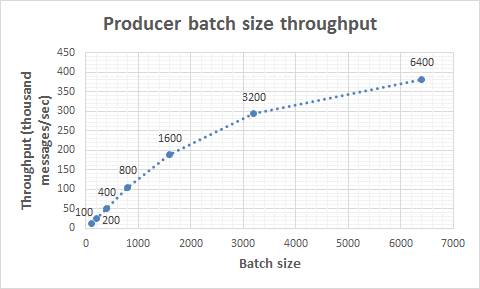
\includegraphics[width=0.8\textwidth]{figures/benchmarks_kafka_batch_2}
\caption{Producer batch size effect on topic throughput}
\label{figure:benchmarks_kafka_batch_2}
\end{figure}

Even though a bigger batch size can increase throughput by orders of magnitude, it also increases the time a message is waits in the producer to be sent in the next batch. Since even a low batch size 100 can achieve greater throughput (12658 messages/sec) than the storm topology in the maximum configuration of our scalability experiment (3988 messages/sec as we will see in Section \ref{section:benchmarks_storm_scalability}), we opt to choose a small batch size in order to reduce message latency. To allow the producer to handle bursts of more packets, we use batch size \textbf{200} for our producer. The rest of the experiments are performed with batch size 200.

\subsection{End-to-End Latency}

Kafka \emph{end-to-end latency} is the time it takes for a message sent by a producer to be delivered to a consumer. For this experiment, the performance tool TestEndToEndLatency creates a producer and a consumer and repeatedly times how long it takes for a producer to send a message to the Kafka cluster and then be received by the consumer. 

The average Kafka end-to-end latency is measured at \textbf{2.871 msec}. Other latency percentiles are presented in Table \ref{table:end-to-end_latency}.

\begin{table}[h!]
\centering
\begin{tabular}{ |c|c| }
\hline
Percentile & Latency (msec) \\ \hline \hline
50th & 2 \\ \hline
99th & 4 \\ \hline
99.9th & 10 \\ \hline
\end{tabular}
\caption{End-to-end latency percentiles}
\label{table:end-to-end_latency}
\end{table}

\subsection{Multiple Producers}

In this experiment we use multiple producers that create messages for a single topic and measure the aggregate message input throughput for the topic. The producers are running on different machines.

Figure \ref{figure:benchmarks_kafka_producers} shows that the aggregate message input throughput increases linearly with the number of the simultaneous producers. This allows us to expand our system to collect and store in Kafka data from multiple different producer sources.

\begin{figure}[h!]
\centering
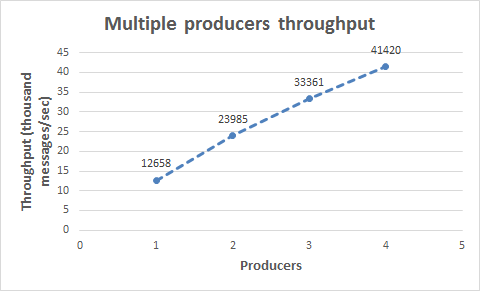
\includegraphics[width=0.8\textwidth]{figures/benchmarks_kafka_producers}
\caption{Topic throughput scalability with the number of producers}
\label{figure:benchmarks_kafka_producers}
\end{figure}

\subsection{Kafka Scalability}

Partitions allow the topic to scale in size by being distributed over the brokers of the cluster and act as the unit of parallelism, providing load balancing over the write and read requests of the producers and the consumers respectively.

To evaluate the scalability of the Kafka topic with the Kafka cluster size, we measure the message input throughput for clusters with different numbers of brokers. The number of the topic's partitions is adjusted according to the number of the brokers.

As we can see in Figure \ref{figure:benchmarks_kafka_scalability} topic throughput scales almost linearly with Kafka cluster size.

\begin{figure}[H]
\centering
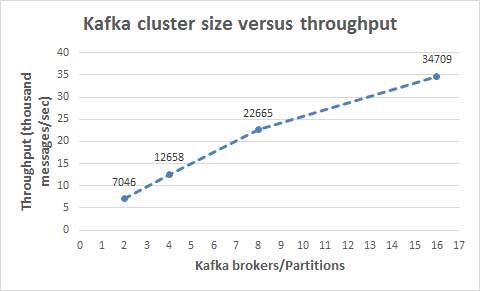
\includegraphics[width=0.8\textwidth]{figures/benchmarks_kafka_scalability}
\caption{Topic throughput scalability with Kafka cluster size}
\label{figure:benchmarks_kafka_scalability}
\end{figure}


\section{Storm Performance Tuning}

The Storm metrics for the following experiments were extracted from the Storm Web UI, which provides information on the running Storm topologies. The CPU metrics were extracted from the Ganglia monitoring system \cite{ganglia} running on the VMs of the evaluation cluster.

\subsection{Parallelism Tuning}\label{subsection:benchmarks_storm_tuning}

To achieve maximum topology throughput, we experiment with the parallelism of its components (spout and bolts). Parallelism tuning in Storm is performed with the help of the capacity metric. 

The \emph{capacity metric} tells us what percentage of the time in the last 10 minutes the bolt spent executing tuples. If this value is close to 1, then the bolt is 'at capacity' and is a bottleneck in our topology. The solution to at-capacity bolts is to increase the parallelism of that bolt. The listing used to compute the capacity metric is:

\begin{lstlisting}[language=C,frame=none]
capacity = (executedTuplesNumber * averageExecuteLatency) / measurementTime
\end{lstlisting}

During the parallelism tuning experiments, when we see that a bolt's capacity is close to 1, we increase its parallelism in the next experiment. We continue tuning until we achieve maximum topology throughput. The parallelism and capacity for each bolt during the parallelism tuning experiments are presented on Table \ref{table:parallelism_tuning}. The name of each experiment denotes the parallelism of each component of the topology: Kafka Spout - Split Fields Bolt - IP to AS Bolt - IP to DNS Bolt - Phoenix Bolt.

Note that capacity is computed based on topology statistics, therefore its value may sometimes appear to be larger than 1. The parallelism of the Kafka Spout is always 4 to match the number of the topic's partitions.

As we can see in Figure \ref{figure:benchmarks_storm_tuning_throughput} we can achieve maximum topology throughput with the parallelism combination \textbf{4-4-4-16-28}. We use these parallelism settings for the rest of the benchmarks.

We also record the average CPU utilization for the Storm and HBase clusters during the tuning experiments and present them in Figure \ref{figure:benchmarks_storm_tuning_cpu}. We notice that the processors of the Storm and HBase clusters are not saturated at maximum topology throughput, which indicates that the topology workload is I/O intensive. This was expected since the IP to DNS Bolt and the Phoenix Blot perform reads and writes respectively to HBase tables.

\begin{table}[h!]
\centering
\resizebox{1\textwidth}{!} {
\begin{tabular}{ |*{9}{c|} }
\hline
\multirow{2}{*}{Experiment} & \multicolumn{2}{|c|}{Split Fields Bolt} & \multicolumn{2}{|c|}{IP to AS Bolt} & \multicolumn{2}{|c|}{IP to DNS Bolt} & \multicolumn{2}{|c|}{Phoenix Bolt} \\ \cline{2-9}
 & Parallelism & Capacity & Parallelism & Capacity & Parallelism & Capacity & Parallelism & Capacity \\ \hline \hline
4-4-4-4-4 & 4 & 0.013 & 4 & 0.011 & 4 & 0.600 & 4 & \textbf{0.987} \\ \hline
4-4-4-12-12 & 4 & 0.021 & 4 & 0.042 & 12 & 0.491 & 12 & \textbf{1.068} \\ \hline
4-4-4-12-20 & 4 & 0.040 & 4 & 0.043 & 12 & \textbf{1.043} & 20 & \textbf{0.911} \\ \hline
4-4-4-16-28 & 4 & 0.043 & 4 & 0.062 & 16 & 0.879 & 28 & \textbf{1.049} \\ \hline
4-4-4-16-36 & 4 & 0.067 & 4 & 0.077 & 16 & 0.816 & 36 & \textbf{1.086} \\ \hline
\end{tabular}
}
\caption{Bolt capacity during parallelism tuning experiments}
\label{table:parallelism_tuning}
\end{table}

\begin{figure}[h!]
\centering
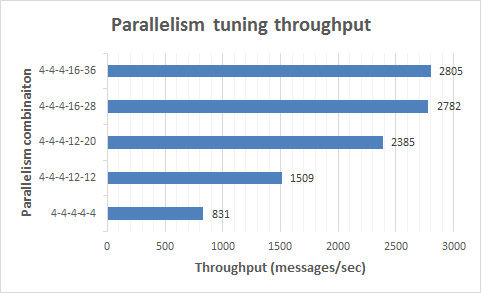
\includegraphics[width=0.8\textwidth]{figures/benchmarks_storm_tuning_throughput}
\caption{Topology throughput during parallelism tuning experiments}
\label{figure:benchmarks_storm_tuning_throughput}
\end{figure}

\begin{figure}[h!]
\centering
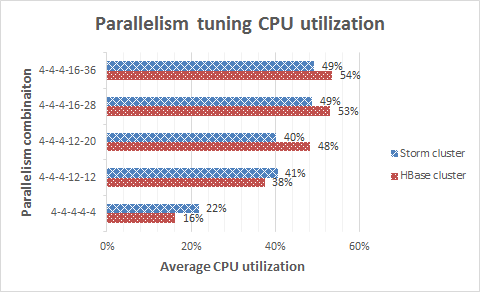
\includegraphics[width=0.8\textwidth]{figures/benchmarks_storm_tuning_cpu}
\caption{Average CPU utilization for the Storm and HBase clusters during parallelism tuning experiments}
\label{figure:benchmarks_storm_tuning_cpu}
\end{figure}

\subsection{Maximum Pending Tuples}

Storm topologies have a \emph{maximum spout pending tuples} parameter. This value puts a limit on the number of tuples that can be in flight (have not yet been acked or failed) in a Storm topology at any point of time. The need for this parameter comes from the fact that Storm uses queues to dispatch tuples from one task to another task. If the consumer side of the queue is unable to keep up with the tuple rate, then the queue starts to build up. Eventually, tuples timeout at the spout and get replayed to the topology, thus adding more pressure on the queues. To avoid this failure case, Storm allows the user to put a limit on the number of tuples that are in flight in the topology. Setting a small maximum pending tuples number can starve the topology from tuples, while a sufficiently large value can overload the topology with a huge number of tuples to the extent of causing failures and replays. 

We experiment with the maximum pending tuples value, while feeding the topology with messages at the maximum rate determined in Subsection \ref{subsection:benchmarks_storm_tuning} (around 2800 messages/sec). The results presented in Table \ref{table:batch_size_throughput} indicate that we can achieve maximum throughput by setting the value of the maximum pending tuples parameter over 100. To allow the topology to handle bursts of more messages, we use the value \textbf{200} for the maximum pending spout tuples parameter. In the case of a message burst, the in-flight tuples will spend more time in the internal queues of the topology, but their number will still be limited by the parameter to avoid failures by overloading.

\begin{table}[h!]
\centering
\begin{tabular}{ |c|c| }
\hline
Maximum pending tuples & Throughput (messages/sec) \\ \hline \hline
10 & 1347 \\ \hline
50 & 2075 \\ \hline
100 & 2782 \\ \hline
200 & 2723 \\ \hline
500 & 2752 \\ \hline
\end{tabular}
\caption{Effect of maximum pending tuples on topology throughput}
\label{table:max_pending_tuples}
\end{table}

\subsection{Bolt Execute Latencies}

A useful metric that allows us to identify the bottlenecks in our topology is the execute latency of each bolt. \emph{Execute latency} is the average time a tuple spends in the execute method of a bolt. 

We record the execute latencies for each bolt of the topology at maximum throughput and present them in Table \ref{table:execute_latencies}. We also compare their relative sizes in Figure \ref{figure:benchmarks_storm_execute_latencies}. It is clear that the tuples spend practically all of their execute time in the IP to DNS Bolt and the Phoenix Bolt. This was expected since these bolts perform reads and writes to HBase tables, while the other bolts execute simple commands in memory.

\begin{table}[h!]
\centering
\begin{tabular}{ |c|c| }
\hline
Bolt & Execute latency (msec) \\ \hline \hline
Split Fields Bolt & 0.047 \\ \hline
IP to AS Bolt & 0.052 \\ \hline
IP to DNS Bolt & 4.779 \\ \hline
Phoenix Bolt & 7.784 \\ \hline
\end{tabular}
\caption{Average execute latency for each bolt of the topology}
\label{table:execute_latencies}
\end{table}

\begin{figure}[H]
\centering
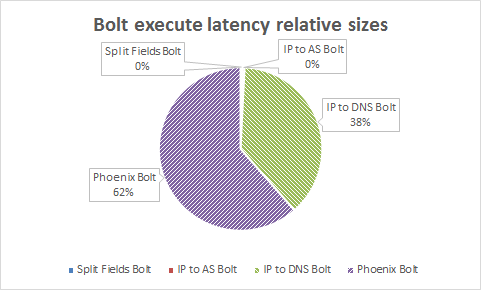
\includegraphics[width=0.8\textwidth]{figures/benchmarks_storm_execute_latencies}
\caption{Relative sizes of execute latencies for the bolts of the topology}
\label{figure:benchmarks_storm_execute_latencies}
\end{figure}

\subsection{Total System Latency}

An important performance indicator for our system is \emph{total system latency}, the time it takes for a message to be sent by the Kafka producer to the topic, consumed by the Kafka Spout, processed by the bolts of the topology and eventually be stored in the Phoenix table and made available for queries.

To compute total system latency we feed the topology with real-time messages and query the table for the row with the latest timestamp. By comparing this timestamp to the current time we can measure the total system latency. Total system latency is measured at \textbf{1.161 sec} on average at maximum topology throughput.

\subsection{Salting Write Performance}\label{subsection:benchmarks_storm_salting}

HBase sequential write suffers from RegionServer hotspotting since the row key is monotonically increasing. Salting the row key provides a way to balance load among the RegionServers, as we described in Section \ref{section:optimizations_salting}.

In this experiment we use a salted and a non-salted table, and compare the throughput of the topology, the write request and CPU utilization on the RegionServers, as well as the execute latency of the Phoenix Bolt. The salted table has 4 salt buckets that are split among the 4 RegionServers of the HBase cluster.

Figures \ref{figure:benchmarks_storm_salting_requests} and \ref{figure:benchmarks_storm_salting_cpu} demonstrate that salting serves its purpose by eliminating write hostspotting. Whereas all the write requests were directed to a single RegionServer for the non-salted table, the load is evenly distributed for the salted table. Note that higher aggregate CPU utilization while using the salted table is linked to better utilization of the cluster's resources, leading to higher topology throughput.

Salting also decreases the Phoenix Bolt's execute latency by \textbf{74\%}, as we can see in Figure \ref{figure:benchmarks_storm_salting_latency}. The execute latency of the Bolt when writing to the non-salted table was increased due to the strain put on the RegionServer that handled all the write requests.

Finally, Figure \ref{figure:benchmarks_storm_salting_throughput} demonstrates that salting massively increases the topology throughput by \textbf{140\%}.

\begin{figure}[H]
\centering
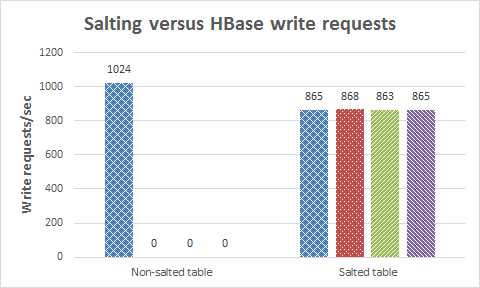
\includegraphics[width=0.8\textwidth]{figures/benchmarks_storm_salting_requests}
\caption{Salting effect on HBase write request distribution}
\label{figure:benchmarks_storm_salting_requests}
\end{figure}

\begin{figure}[H]
\centering
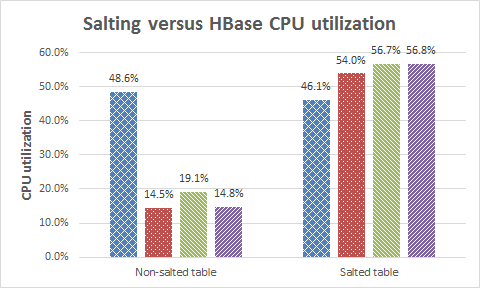
\includegraphics[width=0.8\textwidth]{figures/benchmarks_storm_salting_cpu}
\caption{Salting effect on HBase cluster CPU utilization}
\label{figure:benchmarks_storm_salting_cpu}
\end{figure}

\begin{figure}[H]
\centering
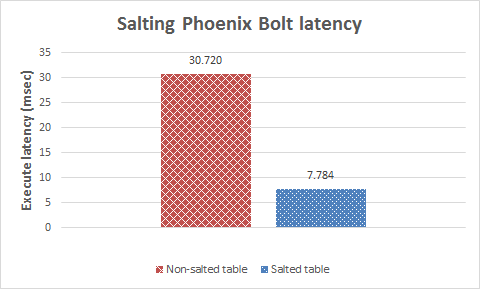
\includegraphics[width=0.8\textwidth]{figures/benchmarks_storm_salting_latency}
\caption{Salting effect on Phoenix bolt latency}
\label{figure:benchmarks_storm_salting_latency}
\end{figure}

\begin{figure}[H]
\centering
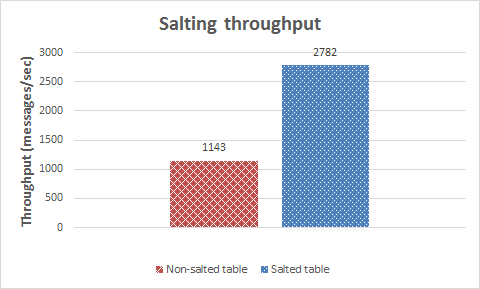
\includegraphics[width=0.8\textwidth]{figures/benchmarks_storm_salting_throughput}
\caption{Salting effect on topology throughput}
\label{figure:benchmarks_storm_salting_throughput}
\end{figure}


\section{Storm Scalability}\label{section:benchmarks_storm_scalability}

To evaluate the scalability of the topology with Storm and HBase cluster size, we measure the topology throughput for different cluster sizes. We increase Storm and HBase cluster sizes simultaneously, meaning that on each test there are as many Supervisors as RegionServers. We also adjust accordingly the number of partitions for the topic, the component parallelism in the topology and the number of salt buckets for the table. After any change to the size HBase cluster we distribute the \texttt{rdns} table evenly among the RegionServers and compact it for data locality.

The topology throughput scalability with Storm and HBase cluster size can be seen in Figure \ref{figure:benchmarks_storm_scalability_throughput}. The average CPU utilization for the Storm and HBase clusters during the scalability experiments is presented in Figure \ref{figure:benchmarks_storm_scalability_cpu}.

\begin{figure}[H]
\centering
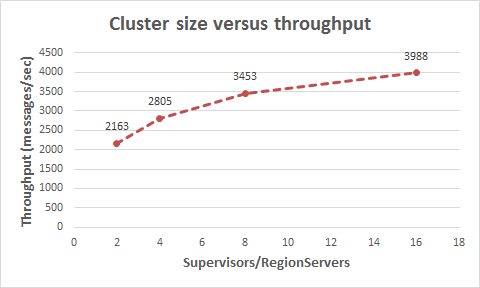
\includegraphics[width=0.8\textwidth]{figures/benchmarks_storm_scalability_throughput}
\caption{Topology throughput scalability with Storm and HBase cluster size}
\label{figure:benchmarks_storm_scalability_throughput}
\end{figure}

\begin{figure}[H]
\centering
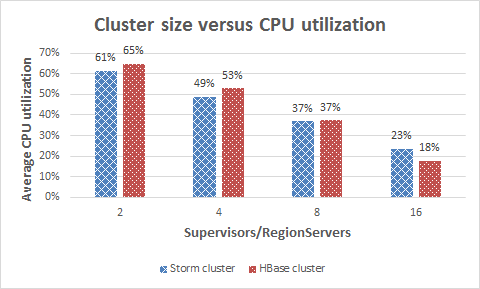
\includegraphics[width=0.8\textwidth]{figures/benchmarks_storm_scalability_cpu}
\caption{Average CPU utilization during scalability experiments}
\label{figure:benchmarks_storm_scalability_cpu}
\end{figure}

We notice that the topology throughput does not scale linearly with Storm and HBase cluster size and the processors are underused for larger cluster sizes. This indicates that the evaluation cluster setup is suffering from disk I/O saturation. As we increase the nodes for each cluster by adding more VMs, the underlying OpenStack cluster infrastructure remains the same, thus the aggregate disk I/O throughput does not increase proportionally with cluster size. This explains the diminishing increases in throughput as we increase the cluster size. If the aggregate disk I/O throughput was increasing according to the cluster size, for example by assigning every node with a dedicated disk, then the topology throughput would then scale linearly with cluster size.


\section{HBase and Phoenix Performance Tuning}

The comparison basis of the following benchmarks is our final Phoenix table, after all optimizations are applied. The table uses Snappy compression and no data block encoding, is split in 3 column families and is salted in 4 buckets. All the tables are compacted and their regions are distributed evenly among the RegionServers. Queries are performed over 10 million rows that are already cached in the BlockCache, unless stated otherwise.

We perform the following two types of queries:

\begin{lstlisting}[language=PhoenixSQL]
SELECT COUNT(*) FROM TABLE netdata;
\end{lstlisting}

The \emph{count} query iterates over the rows of the default column family. This query is useful to measure read performance without any additional calculations.

\begin{lstlisting}[language=PhoenixSQL]
SELECT as.asS, as.asD, COUNT(*) AS pairCount
FROM netdata
GROUP BY as.asS, as.asD
ORDER BY pairCount DESC
LIMIT 10;
\end{lstlisting}

The \emph{topN AS} query returns the top 10 AS pairs in this table ordered by the number of exchanged packets. We also perform the \emph{topN DNS} alternative on some benchmarks, however this query is more computationally intensive, since the \texttt{GROUP BY} clause creates many more distinct pairs for domain names than for autonomous systems. This leads to significantly bigger sets that have to be sorted during the calculations and thus subsequently larger query latency.

\subsection{HDFS Short-Circuit Local Reads}\label{subsection:benchmarks_hbase_short_circuit}

As we described on Section \ref{section:optimizations_short_circuit}, when HDFS short-circuit local reads are enabled, the RegionServer reads local data directly from the disk instead of going through the DataNode. This speeds up data transfer from the disk to the BlockCache when the data is local.

In this experiment we perform a count query over 1 million rows, at first with HDFS short-circuit local reads disabled and afterwards enabled. We measure the total query latency, which includes data transfer time to the BlockCache as well as query processing time. 

When HDFS short-circuit local reads are enabled total query time is reduced by \textbf{62\%}, as we can see in Figure \ref{figure:benchmarks_hbase_short_circuit_latency}.

\begin{figure}[H]
\centering
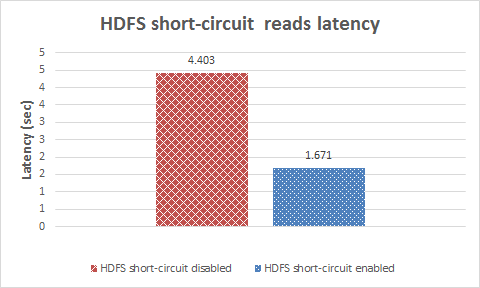
\includegraphics[width=0.8\textwidth]{figures/benchmarks_hbase_short_circuit_latency}
\caption{Enabling HDFS short-circuit for local reads effect on count query latency}
\label{figure:benchmarks_hbase_short_circuit_latency}
\end{figure}

\subsection{Compression and Data Block Encoding}\label{subsection:benchmarks_compression_encoding}

Compression and data block encoding can be used to reduce on-disk data size as well as in-cache data size, as we described in Section \ref{section:compression_encoding}. However this comes with a performance hit for decompression, decoding or both when reading the cached data.

In our experiment we compare on-disk size and in-cache query latency for the following tables:
\begin{itemize}
\item The first table has Fast Diff encoding enabled for all of its column families.
\item The second table has Snappy compression enabled for all of its column families. Compressed BlockCache is enabled.
\item The last table has both Fast Diff encoding enabled and Snappy compression enabled for all of its column families. Compressed BlockCache is enabled.
\end{itemize}

As we can see in Figure \ref{figure:benchmarks_hbase_compression_encoding_size}, using both compression and data block encoding reduces the data size further than the other options. Reduced data size allows more rows can me cached at the same time and reduces data transfer time from the disk to the BlockCache.

However, the best in-cache query latency is achieved by compression alone, as seen in Figure \ref{figure:benchmarks_hbase_compression_encoding_latency}. The data size difference between the second and the third tables is not big enough to outweigh the query latency advantage of the compressed table. This is the reason why we chose compression and no data block encoding for our final table.

\bigskip
\bigskip
\bigskip

\begin{figure}[H]
\centering
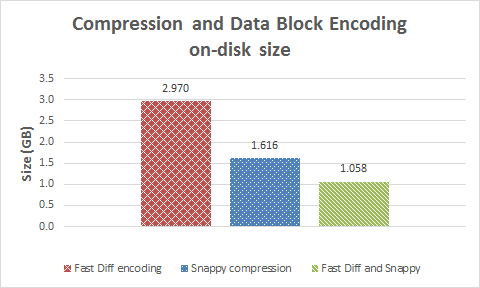
\includegraphics[width=0.8\textwidth]{figures/benchmarks_hbase_compression_encoding_size}
\caption{Compression and data block encoding effect on the on-disk size of a 10 million row table}
\label{figure:benchmarks_hbase_compression_encoding_size}
\end{figure}

\begin{figure}[H]
\centering
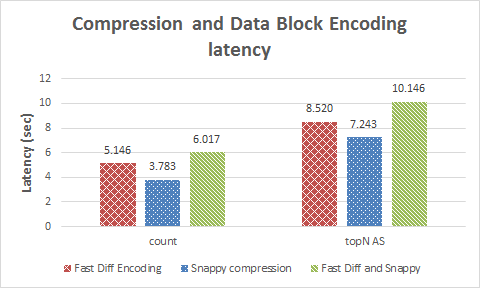
\includegraphics[width=0.8\textwidth]{figures/benchmarks_hbase_compression_encoding_latency}
\caption{Compression and data block encoding effect on query latency}
\label{figure:benchmarks_hbase_compression_encoding_latency}
\end{figure}

\subsection{Number of Column Families}

We compare query performance between our final table, that includes three column families (d, as, dns), and the table containing the same data in one column family. Data is cached by column family, which means that count queries only cache the default family and topN AS queries cache only the as family.

The total size of the final table is divided between the three column families, with the percentages shown in Figure \ref{figure:benchmarks_hbase_cf_sizes}. We measure the total query latency, including data transfer time to the BlockCache, for queries over 1 million rows on the aforementioned tables and present the performance boost that multiple column families offer in Figure \ref{figure:benchmarks_hbase_cf_total_latency}.

\begin{figure}[H]
\centering
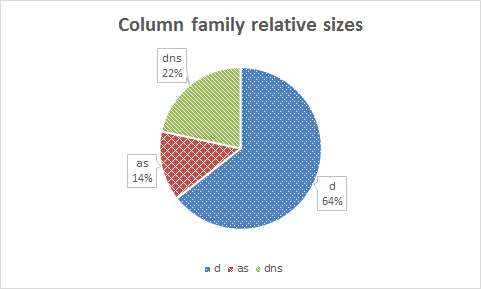
\includegraphics[width=0.8\textwidth]{figures/benchmarks_hbase_cf_sizes}
\caption{Relative sizes of the three column families of the table}
\label{figure:benchmarks_hbase_cf_sizes}
\end{figure}

\begin{figure}[H]
\centering
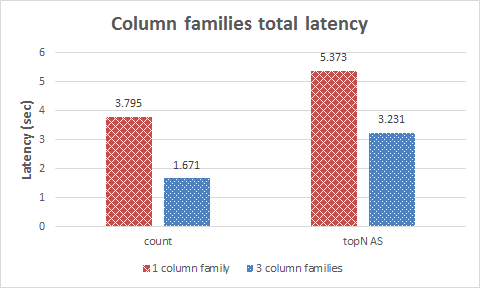
\includegraphics[width=0.8\textwidth]{figures/benchmarks_hbase_cf_total_latency}
\caption{Total query latency for tables with different column family setups}
\label{figure:benchmarks_hbase_cf_total_latency}
\end{figure}

\bigskip

\subsection{Salting Read Performance}\label{subsection:benchmarks_hbase_salting}

As we mentioned in Section \ref{section:optimizations_salting}, aside from write throughput salting can also improve read throughput. Phoenix scans the salted data, sorted within each bucket, in parallel and merge-sorts them at the Phoenix client.

In this experiment we perform a count and a topN AS query on a non-salted and a salted table and compare the query latency. Salting speeds up count and topN AS queries by \textbf{68\%}, as we can see in Figure \ref{figure:benchmarks_hbase_salting_latency}.

\begin{figure}[H]
\centering
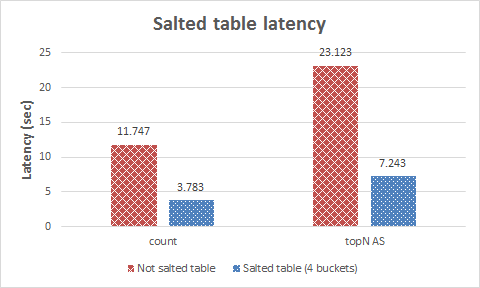
\includegraphics[width=0.8\textwidth]{figures/benchmarks_hbase_salting_latency}
\caption{Salting effect on query latency}
\label{figure:benchmarks_hbase_salting_latency}
\end{figure}


\section{HBase and Phoenix Scalability}

\subsection{Table Rows}

To evaluate the query latency scalability of our table with the size of the data included in the table, we measure the query latency for tables with different numbers of rows. Figures \ref{figure:benchmarks_hbase_rows_latency_1} and \ref{figure:benchmarks_hbase_rows_latency_2} show that the query latency scalability with the size of the data is close to linear.

\begin{figure}[H]
\centering
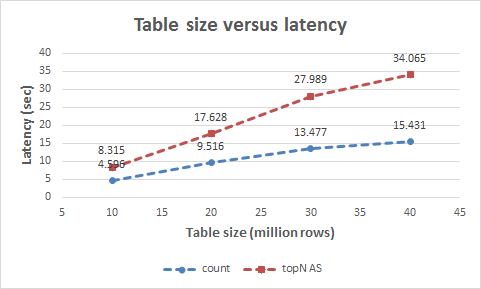
\includegraphics[width=0.8\textwidth]{figures/benchmarks_hbase_rows_latency_1}
\caption{Count and topN AS query latency scalability with table size}
\label{figure:benchmarks_hbase_rows_latency_1}
\end{figure}

\begin{figure}[H]
\centering
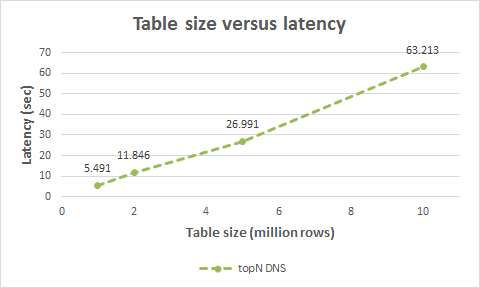
\includegraphics[width=0.8\textwidth]{figures/benchmarks_hbase_rows_latency_2}
\caption{TopN DNS query latency scalability with table size}
\label{figure:benchmarks_hbase_rows_latency_2}
\end{figure}

\subsection{HBase Cluster Size}

To evaluate the scalability of our table with the HBase cluster size, we measure the query latency for clusters with different numbers of RegionServers. The number of the table's salt buckets is adjusted according to the number of the RegionServers. The results of this experiment are presented in Figure \ref{figure:benchmarks_hbase_scalability_latency}.

\begin{figure}[H]
\centering
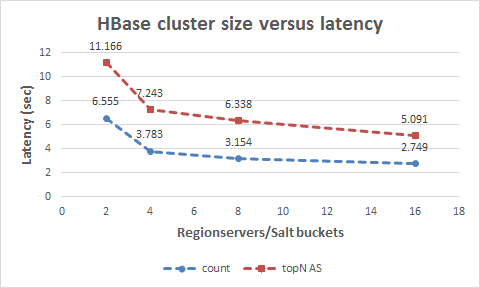
\includegraphics[width=0.8\textwidth]{figures/benchmarks_hbase_scalability_latency}
\caption{Query latency scalability with HBase cluster size}
\label{figure:benchmarks_hbase_scalability_latency}
\end{figure}

\subsection{Multiple Simultaneous Queries}

In this experiment we perform simultaneously the same query from multiple Phoenix clients and measure the average query latency. The clients are running on different machines. 

Figure \ref{figure:benchmarks_hbase_phoenix_clients} shows that multiple queries performed at the same time from different have an additive impact on the average query latency. Since reducing query latency is our priority, multiple simultaneous queries should be avoided.

\begin{figure}[H]
\centering
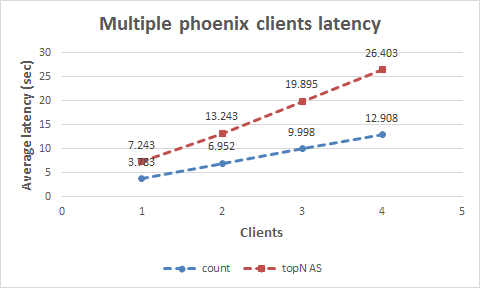
\includegraphics[width=0.8\textwidth]{figures/benchmarks_hbase_phoenix_clients}
\caption{Query latency scalability with the number of Phoenix clients}
\label{figure:benchmarks_hbase_phoenix_clients}
\end{figure}


\cleardoublepage

\chapter{Conclusion}

\section{Concluding Remarks}

TODO

\section{Future Work}

TODO


\cleardoublepage

\end{english}

%%%  Bibliography

\bibliographystyle{plain}
\bibliography{thesis}

%%%  End of document

\end{document}
